\documentclass[12pt, twoside]{report}

%% margins, paper size
\usepackage[a4paper,width=150mm,left=35mm,right=35mm,top=25mm,bottom=25mm,bindingoffset=6mm]{geometry}

%% set up the header and footer area
\usepackage{fancyhdr}
\pagestyle{fancy}
\fancyhead{}
\fancyhead[RO,LE]{\thepage}
\fancyhead[LO]{\leftmark}
\fancyhead[RE]{\leftmark}
\fancyfoot{}

%% no indentation for paragraphs
\setlength{\parindent}{0pt}

\usepackage[utf8]{inputenc}

%% set the graphics path
\usepackage{graphicx}
\graphicspath{ {images/} }

%% for coloring hyperlinks and urls
\usepackage[colorlinks]{hyperref}
\usepackage{breakurl}

%% for sub figure captions
\usepackage{caption}
\usepackage{subcaption}

%% multiple column support
\usepackage{multicol}

%% to draw the uml diagrams
\usepackage{tikz-uml}

%% to use colors
\usepackage{color}

%% draws nice sideways tables
\usepackage{booktabs}
\usepackage{tabularx}
\usepackage[figuresright]{rotating}

%% bibliography setup
\bibliographystyle{plainurl}

\begin{document}

%% preambles

			


\begin{titlepage}
    \begin{center}
        \vspace*{1cm}
        
        \LARGE
        Electronics and Computer Science\\
        Faculty of Physical Sciences and Engineering\\
        University of Southampton\\
        
        \vspace{3.0cm}
        
        \large
        \textbf{Shakib-Bin Hamid}\\
        \today\\
        
        \vspace{2.0cm}
        
        \Huge
        \textbf{Collaborative Consumption for UoS}
        
        \vspace{3.0cm}
        
        \large
        Project supervisor: Dr. Michael R. Poppleton\\
        Second examiner: Dr Nicholas Gibbins\\
        
        
        \vfill
        
        A project report submitted for the award of \\
		MEng Software Engineering
        
    \end{center}
\end{titlepage}
\thispagestyle{plain}
\begin{center}
    \large
    Electronics and Computer Science\\
    Faculty of Physical Sciences and Engineering\\
    University of Southampton\\
        
    \vspace{1.5cm}
    
    \textbf{ABSTRACT}
    
    \vspace{1.5cm}
    
    A project report submitted for the award of MEng Software Engineering
    
    \large
    by \textbf{Shakib-Bin Hamid}
\end{center}

\vspace{1.5cm}
    
\large
The smartphone application industry is diverse and competitive. Emerging technologies and ever-changing user expectations turn the rigid classic engineering principles on its head. On the other hand, modern software engineering practices such as scrum, regular testing, participatory design and user experience evaluation hope to overcome the various challenges that developers usually face in the paradigm. This project demonstrates the application of such processes by developing a hybrid mobile application for University of Southampton students to benefit from Collaborative Consumption.
\chapter*{Declaration}
I am aware of the requirements of good academic practice and the potential penalties for any breaches. I confirm that this project report and accompanying code is all my own work except the open-source frameworks and libraries in Appendix \ref{appendix:libs}, which are referenced and credited in the report and code.
\chapter*{Acknowledgements}
I want to thank my parents, Mr Abdul Hamid and Mrs Dilshad Begum, for always supporting me, my project supervisor, Dr Michael Poppleton, for his directions in the project and finally, Miss Rosanna Lathwell for designing my app logo.

%% content list
\tableofcontents
\listoffigures
\listoftables

%% main body
\chapter{Introduction}

Technology has introduced new trading concepts that can expand a traditional sharing community far beyond that of close friends. Take eBay for example - an eBay user can post the items that they want to sell or put on auction,  with name, description and pictures to help a buyer minimise the risks in transactions. A buyer can also find ratings-reviews about the seller's previous transactions etc. Both buyer and seller can securely pay via Paypal with buyer protection. These technology platforms themselves are not providing any items; they are not product brands. Rather, they provide some features that build trust in their communities, because sharing, swapping, renting etc. only happens when there is trust between the participating parties. Such Sharing Economy using technology is called \textit{Collaborative Consumption} (CC).\\

University of Southampton (UoS) itself has a vibrant student community. Students here borrow calculators and books for the odd coursework, parking spots for their visiting parents, sell or give away their old mobiles, music players or laptops etc. This happens often enough that there are several social media groups for sharing items. A targeted Collaborative Consumption tool for UoS students can certainly thrive because of the existing communities. This tool needs to be mobile because an average student usually accesses the aforementioned social media sites from their phones, on the go.\\

However, the goal of this project is not promoting CC, rather it is to explore modern software engineering practices - 

\begin{description}
	\item [scrum] : develop in short, targeted and self contained cycles,
	\item [participatory design] : include end users in requirements elicitation and user experience testing,
	\item [user centred development] : develop towards user stories rather than use cases,
	\item [behaviour driven development] : write automated test scripts for each user story under preconditions.
\end{description}

Another goal is to experience both \textit{server} and \textit{client} side development to demonstrate how mobile application features such as push notifications etc. operate. The premise of a mobile CC tool is suitable to demonstrate such processes.\\

Mobile applications for smartphones usually target a wide range of users from very different backgrounds. So, evaluating User Experience (UX) for these applications is essential and time should be spent on user participations. However, development in the native language for a platform, Java on Android for example, usually requires a very steep learning curve. Together with the need to develop a full stack application in such a short time, a fast mobile development framework is required. Such tools exist that it is possible to build mobile applications entirely in JavaScript (both server and client) and deploy the same code to multiple platforms. As this project's resultant application is a proof-of-concept rather than a marketplace application, it is quite acceptable and even preferred to work with such \textit{Hybrid} solutions.\\

Overall, the goal of this project is to demonstrate modern Software Engineering practices by implementing a Client Hybrid Mobile Collaborative Application and the corresponding Server Application.\\

Below is a summary of what content is to follow -

\begin{description}
	\item [Chapter 2] reviews the relevant literature on collaborative consumption, hybrid mobile development and agile software development practices.
	\item [Chapter 3] lists the features of the client app and discusses what features were discarded and why.
	\item [Chapter 4] explains how the project was organised/structured and managed during different stages such as sprints etc.
	\item [Chapter 5] gives an overview of the technologies used and discusses the architecture of the system as a whole.
	\item [Chapter 6] explains the client and server implementation in-depth.
	\item [Chapter 7] discusses how the implementation was tested - automated and against scenarios.
	\item [Chapter 8] gives a detailed description of why and how the user sessions were organised, performed and documented.
	\item [Chapter 9] evaluates the success, shortcomings and usefulness of the project.
	\item [Chapter 10] concludes the project aims and results.
\end{description}
\chapter{Literature Review}
\label{chap:lit}
%%%%%%%%%%%%%%%%%%%%%%%%%%%%%%%%%%%%%%%%%%%%%%%%%%%%%%%%%%%%%%%%
%% Literature review for CC

\section{Collaborative Consumption}

\subsection{Defining CC}
\textit{"Collaborative Consumption (CC)"} is people, in a community, acquiring or distributing physical goods or services for \textit{some form of compensation} amongst themselves \cite{Belk:2014}. The form of compensation dictates whether the transaction can be labelled as \textit{Sharing} ownership, \textit{Swapping or Trading} for another resource or even \textit{Buying and Selling} of used goods. One commonality in all such practices is the interaction amongst the community members using technology, especially Web 2.0 (otherwise known as the \textit{interactive Web}). Sharing items within a small organisation like family or friends has been present in society for a very long time, but the technologies like social networks, e-commerce etc. available today allow people to make trusted transactions in large communities. In fact, the CC platforms are merely \textit{"economical-technological coordination providers"} \cite{Hamari:2015}. In other words, people have been willing to engage in 'Sharing Economy' if a suitable technological platform exists.\\

\subsection{CC Categories}
There are three categories of Collaborative Consumption \cite{Albinsson:2012} :

\begin{itemize}

	\item Where consumers pay for using a resource. For example: Singapore based \href{http://www.rent-that-toy.com}{Rent-A-Toy} rents expensive toys for a fee.
	
	\item Where members redistribute their rarely used or unwanted items. For example: \href{http://www.heyneighborapp.com}{Hey, Neighbor!} is a site where those in particular locales can share/rent their equipment and 'micro-favours'.
	
	\item Where people share less tangible resources like skills, space, time etc. For example: \href{https://www.airbnb.co.uk}{Airbnb} and \href{https://www.couchsurfing.com}{Couchsurfing} members temporarily share their living space with fellow members.

\end{itemize}

On the other hand, two categories of Collaborative Consumption exchanges are \cite{Hamari:2015} - 

\begin{itemize}

	\item \textbf{\textit{Access over ownership}}: When a user offers and shares their resources for a limited time to another user in the community (with or without the need for an  exchange). For example: \href{https://www.renttherunway.com}{Rent the Runway} rents expensive designer cloths to people for a fee or \href{https://www.yourparkingspace.co.uk}{Your Parking Space} lets the users to list their parking space to be available to rent to others.
	
	\item \textbf{\textit{Transfer ownership}}: When a user completely relinquishes their claim on an item and gives it away to another (also with or without the need for an  exchange). For example: \href{http://www.swapstyle.com}{Swapstyle} lets its users swap their cloths. 

\end{itemize}

\subsection{Reasons to Participate}
Four possible reasons why people take part in Collaborative Consumption \cite{Hamari:2015} are - 

\begin{itemize}

	\item \textbf{\textit{Sustainability}}: People want to reuse and recycle their owned goods to bring wastage to a minimum and sustain a better environment.
	
	\item \textbf{\textit{Enjoyment}}: Users often enjoy sharing their produced item because it can help others. For example: Many software developers give away their software source code on \href{https://github.com}{Github} because they enjoy software freedom.
	
	\item \textbf{\textit{Reputation}}: Users enjoy the earned reputation in the community from participating in many transactions. For example: Well traded \href{http://www.ebay.co.uk}{Ebay} users usually carry out more successful transactions.
	
	\item \textbf{\textit{Economic Benefits}}: Members want to save some cost by swapping their items, buying used ones or earn some money by selling unwanted goods.
	
\end{itemize}

The followings affect the satisfaction of a sharing option \cite{Mohlmann:2015}-
\begin{itemize}

	\item \textbf{\textit{Cost Savings}}: A sharing option that saves some money for the consumer leads to a successful transaction more often.
	
	\item \textbf{\textit{Familiarity}}: Consumers trade more often on Collaborative Consumption platforms that they are familiar with (through exposure from various media).
	
	\item \textbf{\textit{Service Quality}}: Members use Collaborative Consumption platforms that give them easy options, suggestions and an overall better experience.
	
	\item \textbf{\textit{Trust}}: People only want to carry out transactions if they feel that the community is secure, welcoming and the members are trustworthy.
	
\end{itemize}

\subsection{Collaborative Consumption in UoS}
University of Southampton students also have a Facebook Group called \href{https://www.facebook.com/groups/302702106480967/?fref=ts}{Free \& For Sale}, where students put up their unwanted item to sell, swap or give away. These items can include calculators, books, cloths, fashion accessories, furniture, kitchen tools, garage tools, event tickets, transport tickets, mobiles, laptops, electronic boards etc. Students arrange the transactions within themselves. The group has been quite successful in recent years.\\

The above leads me to believe that University of Southampton students can truly benefit from a Collaborative Consumption platform which lets \textit{only} them trade on the platform and integrates with their campus identity. There are existing platforms including \textbf{Ebay}, \textbf{Gumtree} and \textbf{Facebook} where students can co-ordinate their transactions. But none of these are suited for this particular atmosphere and cannot provide support for a UoS community.

%%%%%%%%%%%%%%%%%%%%%%%%%%%%%%%%%%%%%%%%%%%%%%%%%%%%%%%%%%%%%%%%



%%%%%%%%%%%%%%%%%%%%%%%%%%%%%%%%%%%%%%%%%%%%%%%%%%%%%%%%%%%%%%%%
%% Literature review for Hybrid Dev

\section{Hybrid Mobile Development}

\subsection{Mobile Applications}

\textbf{Native} apps are those built using platform specific tools, for example: Swift or C\# and XCode for iOS, Java (Dalvik runtime) and Android Studio for Android etc. Examples are - Gmail by Google, Pages by Apple etc.\\

\textbf{Web} apps are built using HTML, CSS and JavaScript and hosted on a \textit{website} that can be accessed from any browser including a mobile. Examples are - Netflix website or Google Docs etc.\\

\textbf{Hybrid} apps sit between native and web apps (Figure \ref{Figure:Hybrid} \cite{salesforcehybrid-site}). They are built using similar technologies as web apps, but are then compiled into platform specific installers and used as a native app. Underneath the surface, these apps usually run a \textit{localhost} server on the mobile that runs the app and the OS accesses them using web-view. \cite{Litayem:2015, Karadimce:2014}

\begin{figure}[!h]
  \centering
    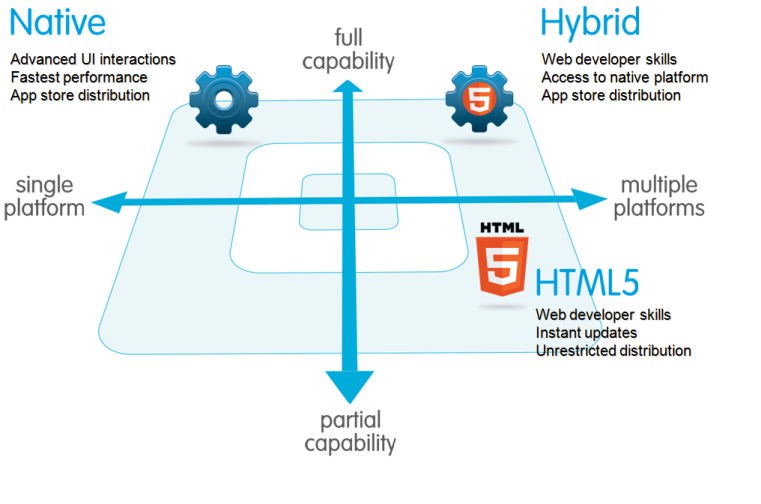
\includegraphics[width=0.6\textwidth]{hybrid-a}
  	\caption{Hybrid Apps}
  \label{Figure:Hybrid}
\end{figure}

\subsection{Advantages of Hybrid Apps}

A major difficulty in native development is that, it easily becomes difficult to simultaneously develop, maintain and support for different platforms \cite{Litayem:2015}. Very little of one device's code can be ported over to another because of lack of standards, e.g. the standard Android uses commas to separate items in a list, but Samsung phones use a semicolon \cite{Joorabchi:2013}. Whereas, a hybrid app can be ported into multiple platforms simultaneously, with very little (if any) change.\\

Native apps usually perform better than their web and hybrid counterparts because they can leverage the full potential of the OS. While web apps have a disadvantage of being accessible only over network and are slow to respond, recent hybrid app development frameworks have started hardware acceleration. In fact, apart from 3D games, there is negligible or unnoticeable performance gap between the two paradigms \cite{Charland:2011}.\\

Early web and hybrid apps were notorious for their lack of usability on a mobile, because the components such as buttons were not optimised for touch. Modern frameworks, however, provide the exact components as the native apps. Resultantly "end users value hybrid and native apps similarly" \cite{Malavolta:2015}.

\subsection{Challenges in Hybrid Apps}

Lack of automated testing frameworks is a major drawback for production ready hybrid apps. The mobile app industry, in general, does not have a unified testing pattern for either usability or functional testing \cite{Joorabchi:2013}. Each OS provider has its own IDE (Integrated Development Environment) and test environment. But most hybrid frameworks, being very recent and open-source, do not have such features.\\

Moreover, debugging is difficult in mobile apps, in general, because CPU, memory etc. monitoring is cumbersome, even impossible at times. This is specially true in hybrid frameworks, as most only support primitive emulation rather than a debugger.\\

Finally, security is an emerging issue. Being built on web technologies, it is subject to threats from that paradigm as well as mobile OS threats \cite{Brucker:2016, Hale:2015}.\\

Nevertheless, I believe hybrid technologies are perfect for a short project with intentions of fast prototyping and user evaluation.

%%%%%%%%%%%%%%%%%%%%%%%%%%%%%%%%%%%%%%%%%%%%%%%%%%%%%%%%%%%%%%%%



%%%%%%%%%%%%%%%%%%%%%%%%%%%%%%%%%%%%%%%%%%%%%%%%%%%%%%%%%%%%%%%%
%% Literature review for Scrum

\section{Agile Development \& Scrum}

\subsection{Overview of Agile Method}

The “Agile Manifesto" \cite{beck:2001} stated four core principles - 

\begin{enumerate}
	\item \textbf{Individuals and interactions} over processes and tools
	\item \textbf{Working software} over comprehensive documentation
	\item \textbf{Customer collaboration} over contract negotiation
	\item \textbf{Responding to change} over following a plan
\end{enumerate}

Put simple, agile software development is to - define a vision and scope for the project, define requirements together with customer, build in iterations and review the results with the customer to update the requirements until release \cite{Inayat:2015}. This iterative framework is called \textbf{Scrum}.

\subsection{Scrum}

In Scrum framework, the development team works closely with the \textbf{Product Owner} (usually the customer). The team defines requirements in forms of \textbf{User Stories} (\texttt{As a <user>, I want <feature> so that <reason>} \cite{Rees:2002}); how the task is carried out is left open. The project is broken down into iterations (typically 1-4 weeks), each with a goal such that the vision of the project is fulfilled by the release period \cite{Schwaber:1997}.\\

The long list of tasks is called the \textbf{Product Backlog}. At each iteration, tasks are selected (\textbf{Sprint Backlog}) to generate a \textit{working} software of \textit{value} to the customer. This is then demonstrated to the product owner and shippability is discussed. Backlog is updated and prioritised with possibly new or reduced items (Figure \ref{Figure:scrum} \cite{Schwaber:1997}), changing the direction and contents of future deliveries. The development team also has a \textbf{Review} meeting to improve internal development process.\\

\begin{figure}[!h]
  \centering
    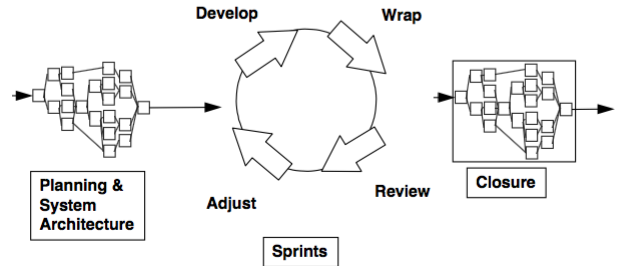
\includegraphics[width=0.6\textwidth]{scrum}
  	\caption{Scrum}
  \label{Figure:scrum}
\end{figure}


However, agile methods are not perfect by any means. For example: it is not always possible to make upfront cost estimation because of the volatile nature of development \cite{Ramesh:2010}. As always, an early architectural design decision may adversely affect future development. Despite these, I think it is preferable to take an agile approach to any modern mobile app development \cite{Wasserman:2010} because of the nature of the industry itself.

\section{Testing in Modern SE}
\label{sec:testing}

\subsection{Test Driven Development}

Test Driven Development (TDD) is a software engineering practice where automated unit tests are written before development. These tests fail at first, but start to pass as the development proceeds. Thus development itself remains focused and targeted \cite{Williams:2003}. It is also a part of Extreme Programming (XP). Modern agile teams believe that the advantages include \cite{George:2004} - 

\begin{itemize}
	\item Efficiency in error detection in later stages because of comprehensive development stage testing.
	\item Fast regression testing possible because of the test driven code.
	\item Testability (code that is easy to test) increases in the entire codebase.
	\item Loosely coupled system as a result of the need for mock objects.
\end{itemize}

However, some shortcomings of the TDD process are \cite{George:2004} - 

\begin{itemize}
	\item Some code is inherently difficult to unit test, for example: GUIs etc.
	\item The code must coherently support mock objects to isolate other code which proves hard in practice.
	\item Testing hard-to-test code needs a certain level of experience and determination.
\end{itemize}

In the literature, I have found TDD to be the current trend across the industry, including myself using the process in IBM during internship. However, TDD requires an experienced team in the required technology to implement the architecture and have a coherent data model. In short projects it can actually be counter productive.

\subsection{Behaviour Driven Development}

In TDD most developers are unsure what and how much to test, where to start etc. There is also usually a gulf between developer testing and customer acceptance. Behaviour Driven Development (BDD) attempts to answer these questions by mandating automated test cases based \textit{only} on the user stories \cite{Solis:2011}. Any other automated test is optional for the development teams. Below is a test structure for BDD, extracted from a user story - 

\begin{center}
\texttt{\textbf{Given} <init\_context>}\\
\texttt{\textbf{When} <event> occurs}\\
\texttt{\textbf{Then} <assert\_outcome>}
\end{center}

This style can be placed in between unit and integration tests in traditional testing. One major advantage is that it is easier to understand as a customer. BDD may or may not replace general unit testing itself. Also, regression testing mandatory as usual.
\chapter{Application Specifications}

In this chapter, I have listed the features of the Client app, as well as which features were discarded and justifications for doing so.

\section{Implemented Features}

Using this app, students can borrow (with or without a deposit) and sell items amongst themselves (Figure \ref{fig:lend}). They can search for their desired item from a list (Figure \ref{fig:homepage}) via text based search (Figure \ref{fig:search}) or from a list of categories (Figure \ref{fig:category}) as well as add their own items with textual details and pictures (Figure \ref{fig:add}, \ref{fig:gallery-select}). Users can navigate the app using a slide-in menu to other pages (Figure \ref{fig:menu}), e.g. their profile where they find their avatars, simple ratings, items and comments by others (Figure \ref{fig:profile}). They also receive push notifications about items they want to borrow/sell and find a list of such notifications in app (Figure \ref{fig:notification}, \ref{fig:requests}).

\section{Unimplemented Features}

This project is not about creating a production ready app, but rather to investigate and experience software engineering(SE) practices. If some feature did not add to a high-priority user story or did not add to the SE values, then it was ignored. Some of the important ones are below - 

\begin{itemize}
	\item Users cannot create their own accounts, i.e. there is no registration.  One reason to do so is that, I imagined such a system to use the university authentication to guarantee that only UoS students use the service. Although, there is a REST route available on the server side to do it, so that, on the first login in a production app, a User object will be created on the database.
	
	\item There is no chatting option on the app, even though the placement in the UI is there. The major reasons are - time constraints and less priority. Given the choice between push notification and chat, the user interviews led me to (rightly) prioritise push. I discuss more about it in later chapters.
	
	\item Users cannot upload a profile picture, a default one is set for them. For demo purposes, I edited user objects on the database myself in the figures here. I have demonstrated how such features can be implemented by allowing to upload item picture, so other user stories took priority.
\end{itemize}

\section{Screenshots}
\begin{figure}[!h]
    \centering
    \begin{subfigure}[b]{0.3\textwidth}
        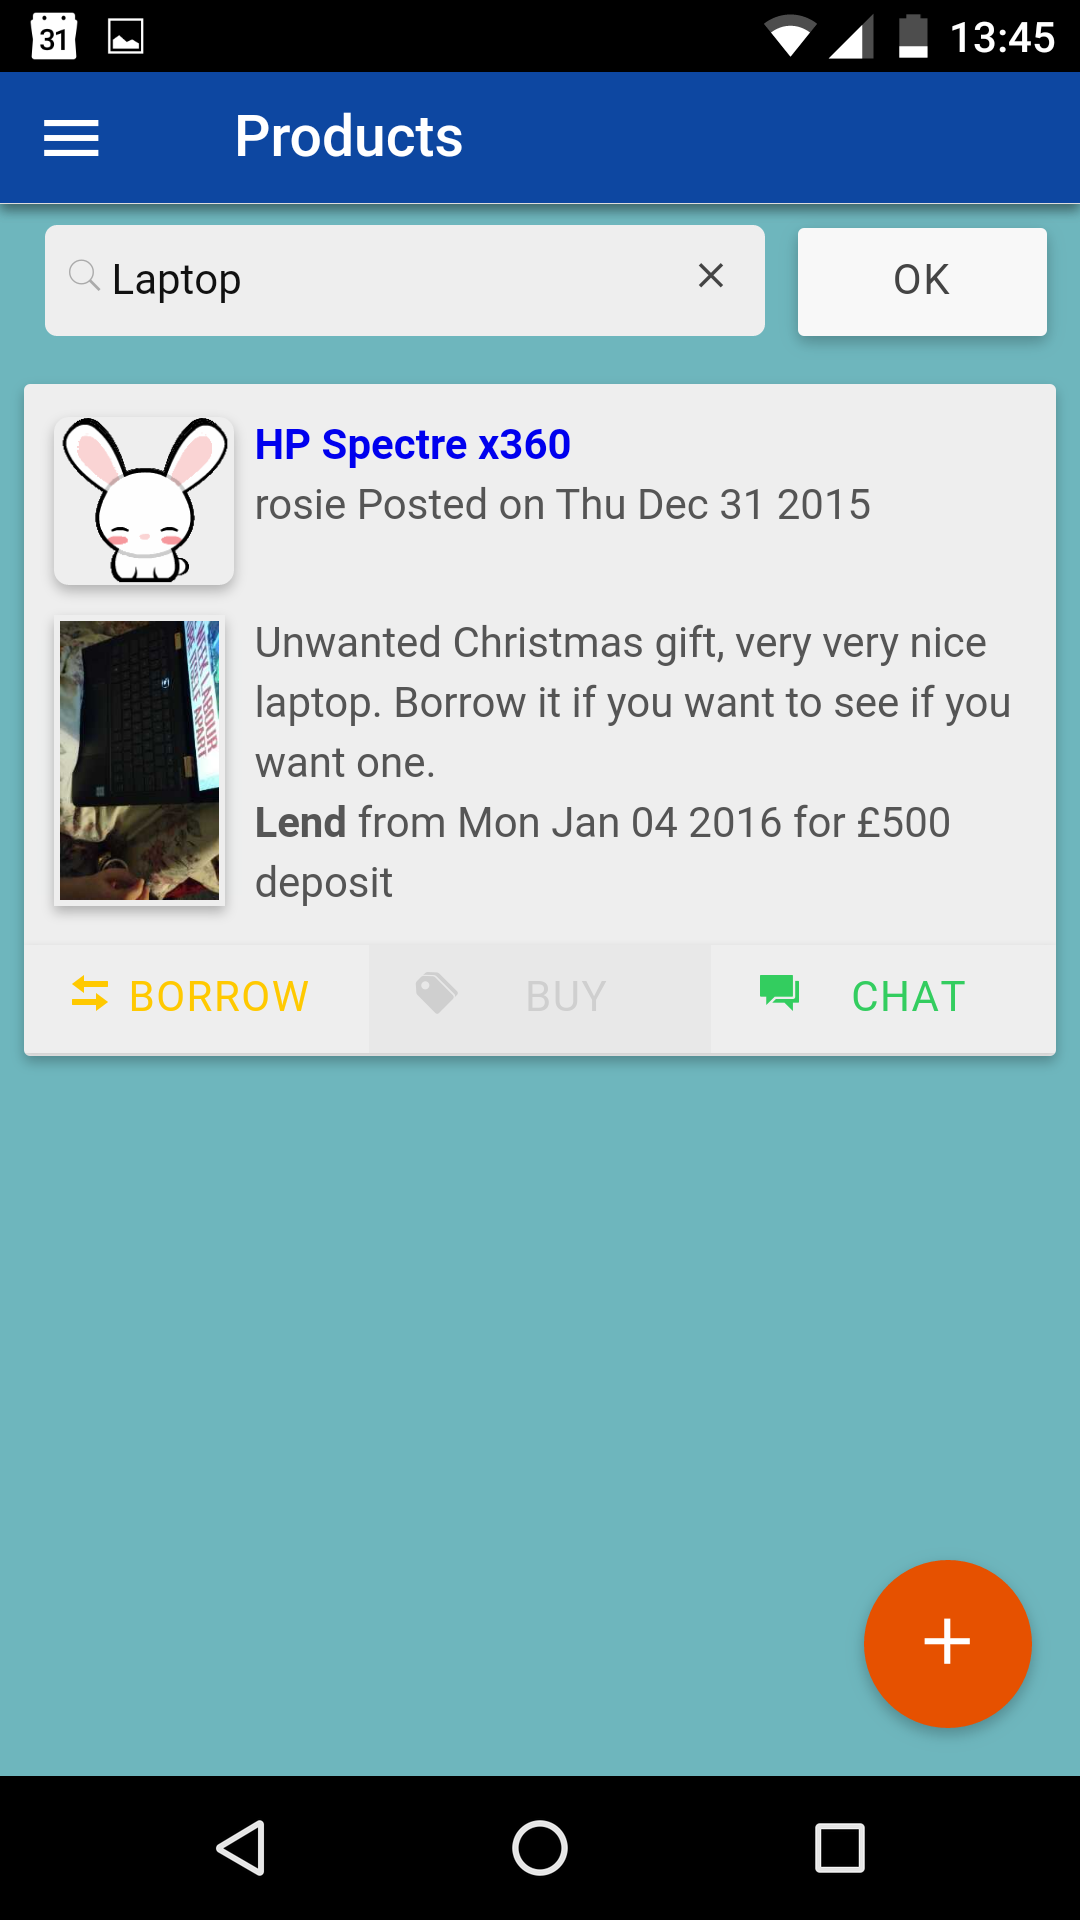
\includegraphics[width=\textwidth]{search}
        \caption{Search}
        \label{fig:search}
    \end{subfigure}
    ~
    \begin{subfigure}[b]{0.3\textwidth}
        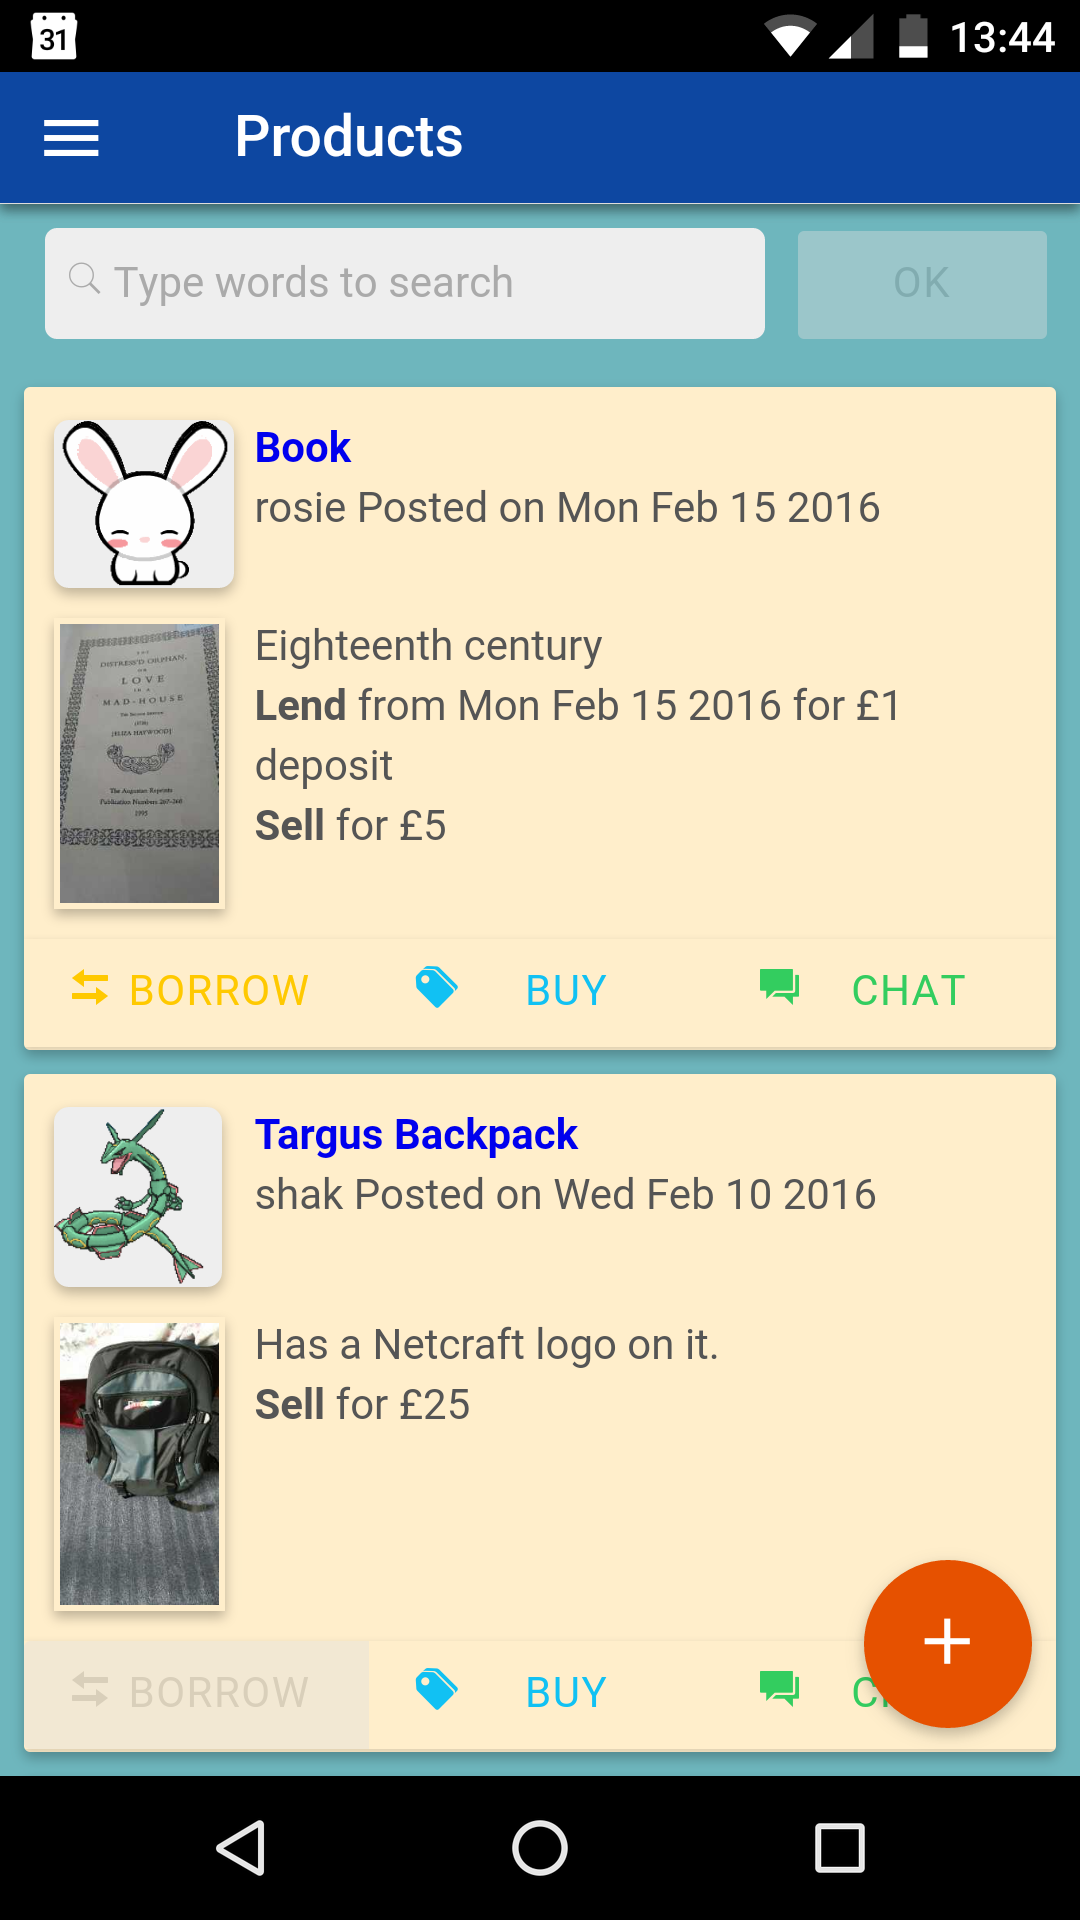
\includegraphics[width=\textwidth]{homepage}
        \caption{Product List}
        \label{fig:homepage}
    \end{subfigure}
    ~
    \begin{subfigure}[b]{0.3\textwidth}
        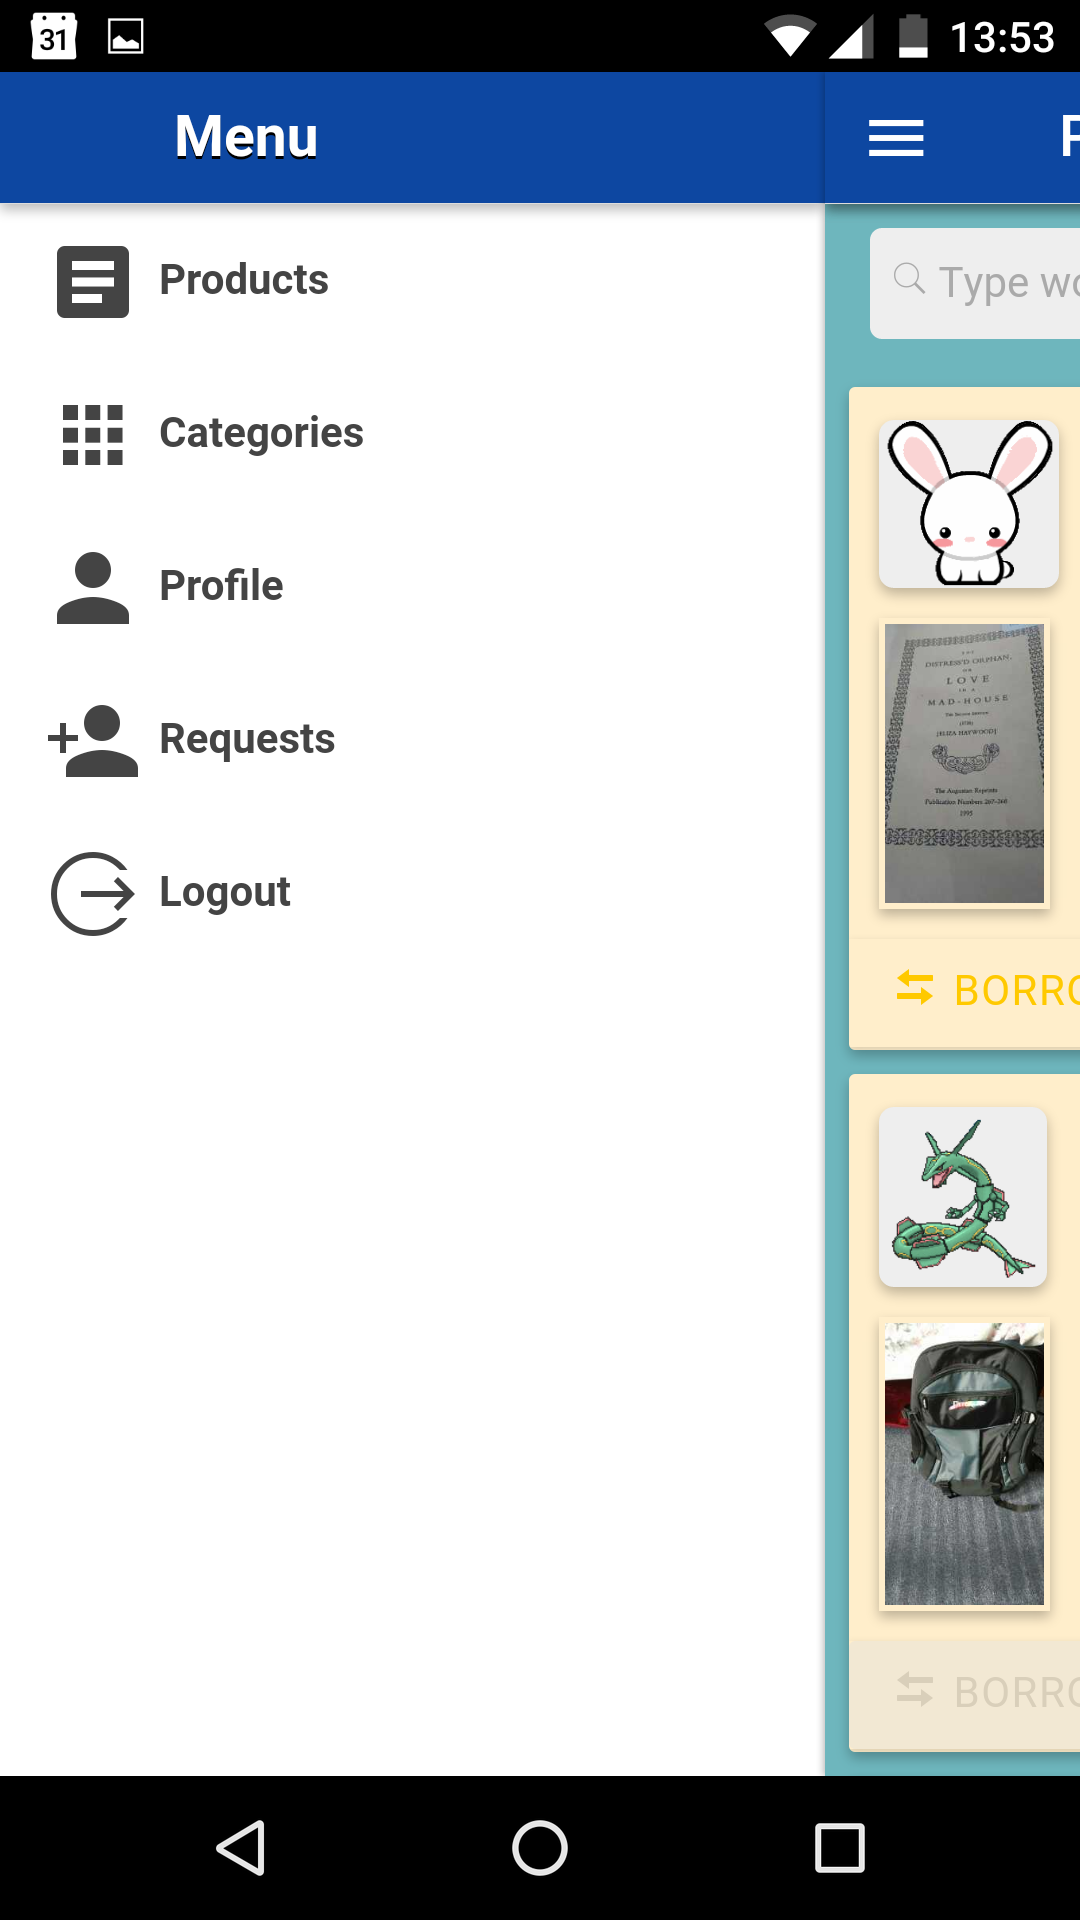
\includegraphics[width=\textwidth]{menu}
        \caption{Menu}
        \label{fig:menu}
    \end{subfigure}
    \caption{Screenshots}\label{fig:scr3}
\end{figure}
\begin{figure}[!h]
    \centering
    \begin{subfigure}[b]{0.3\textwidth}
        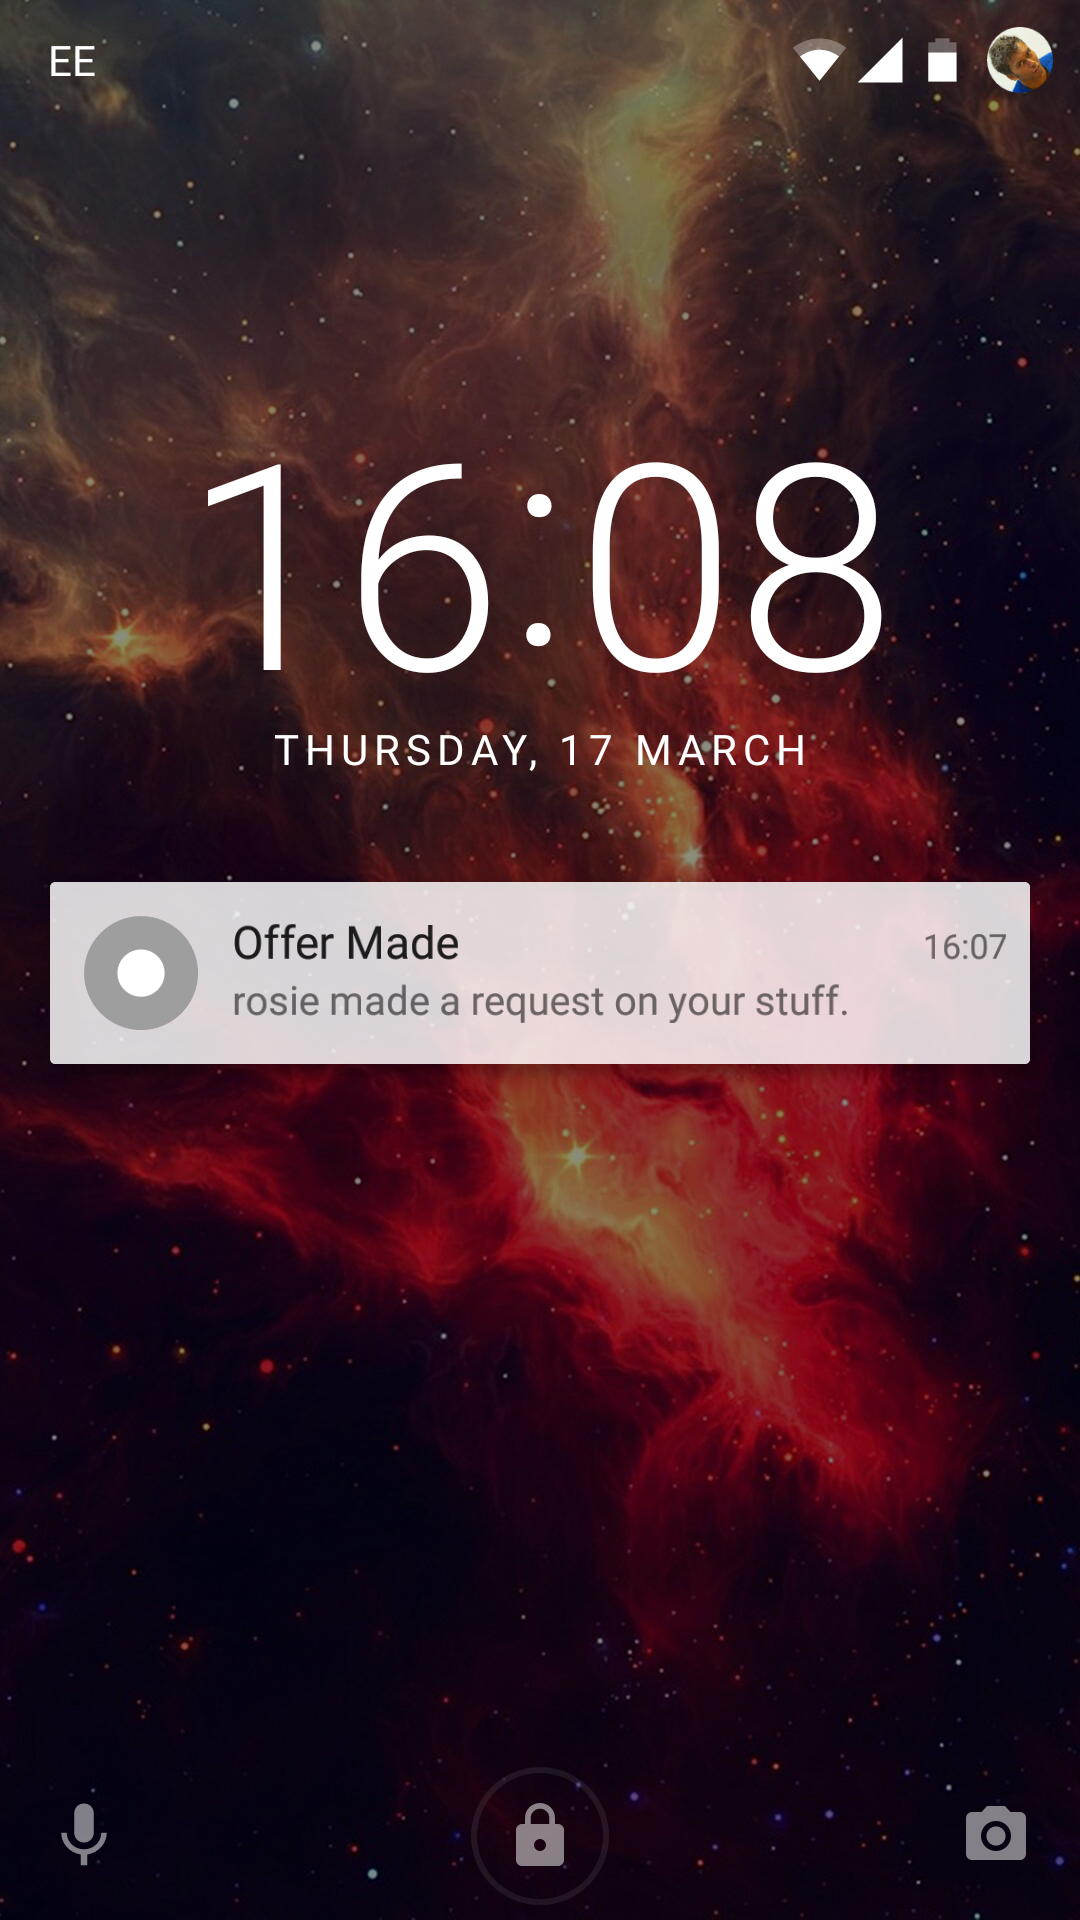
\includegraphics[width=\textwidth]{notification}
        \caption{Notification}
        \label{fig:notification}
    \end{subfigure}
    ~
    \begin{subfigure}[b]{0.3\textwidth}
        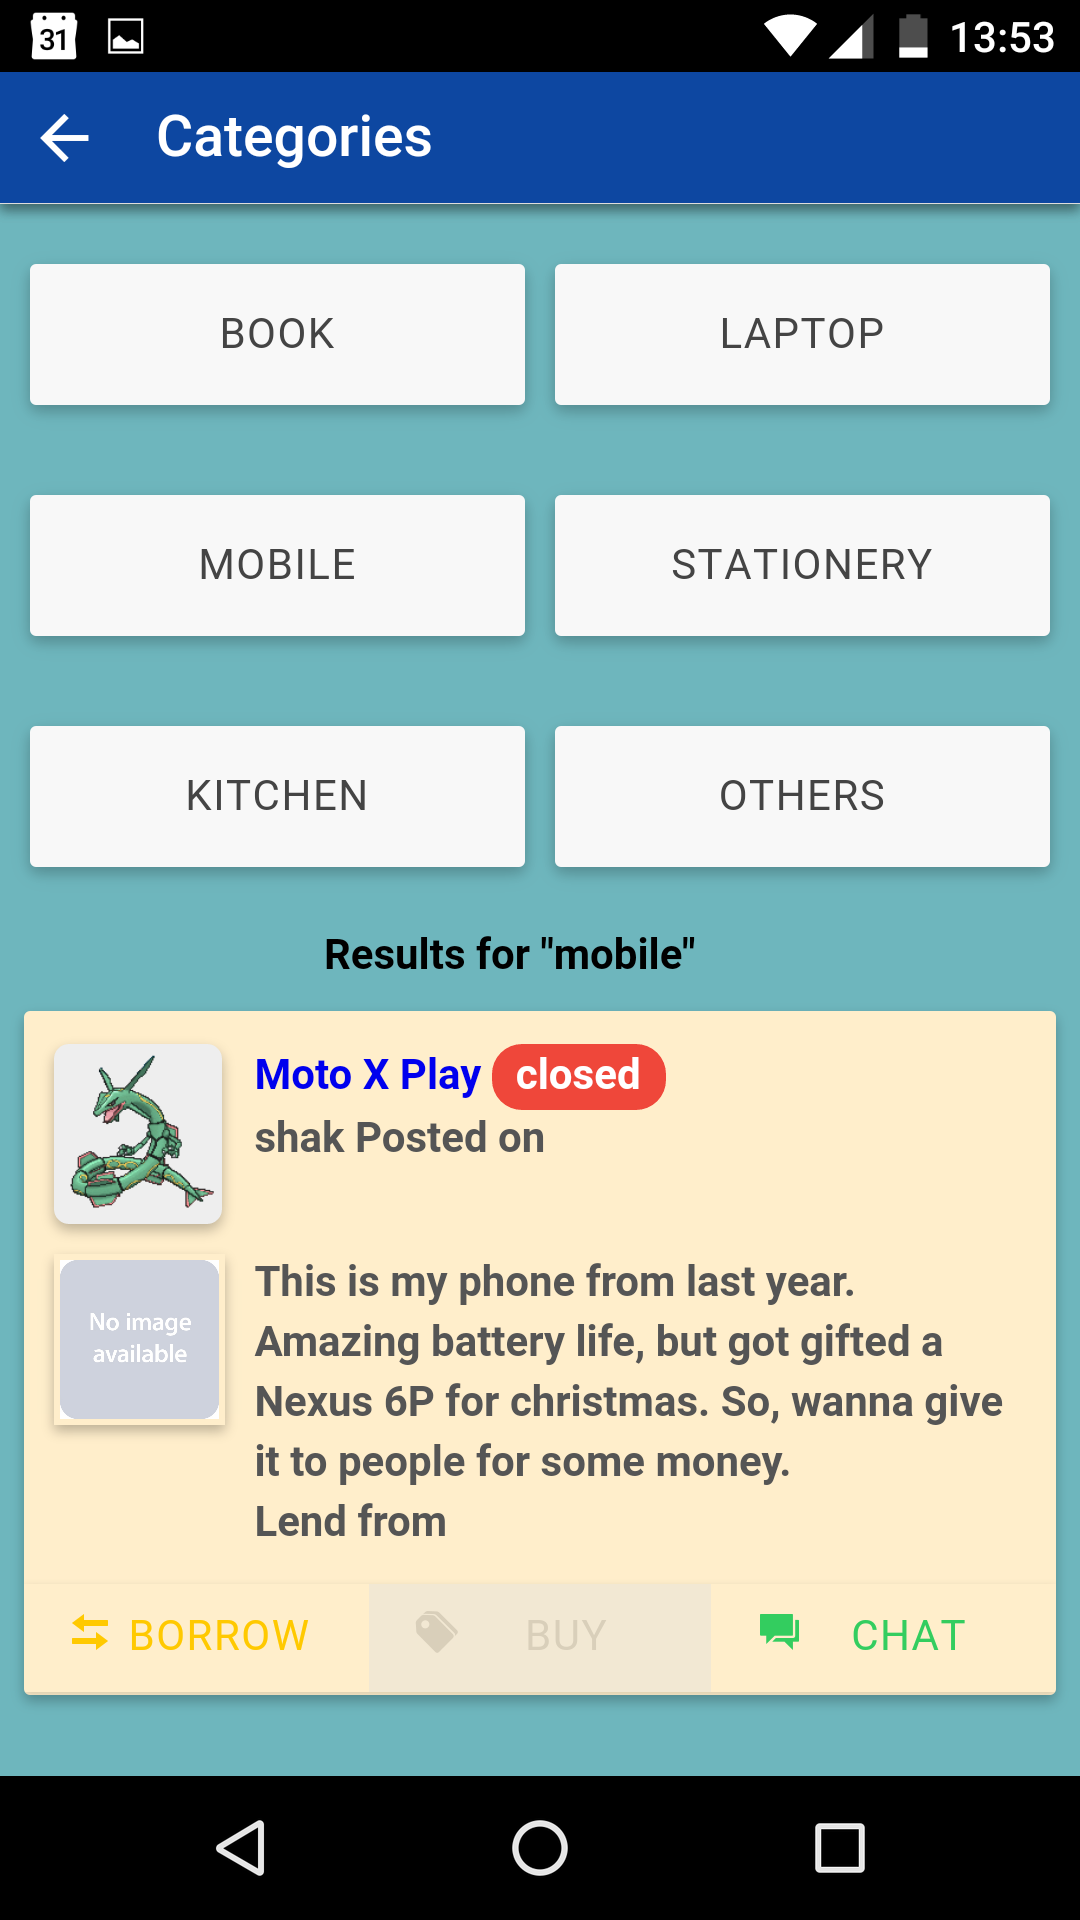
\includegraphics[width=\textwidth]{category}
        \caption{Category List}
        \label{fig:category}
    \end{subfigure}
    ~
   \begin{subfigure}[b]{0.3\textwidth}
        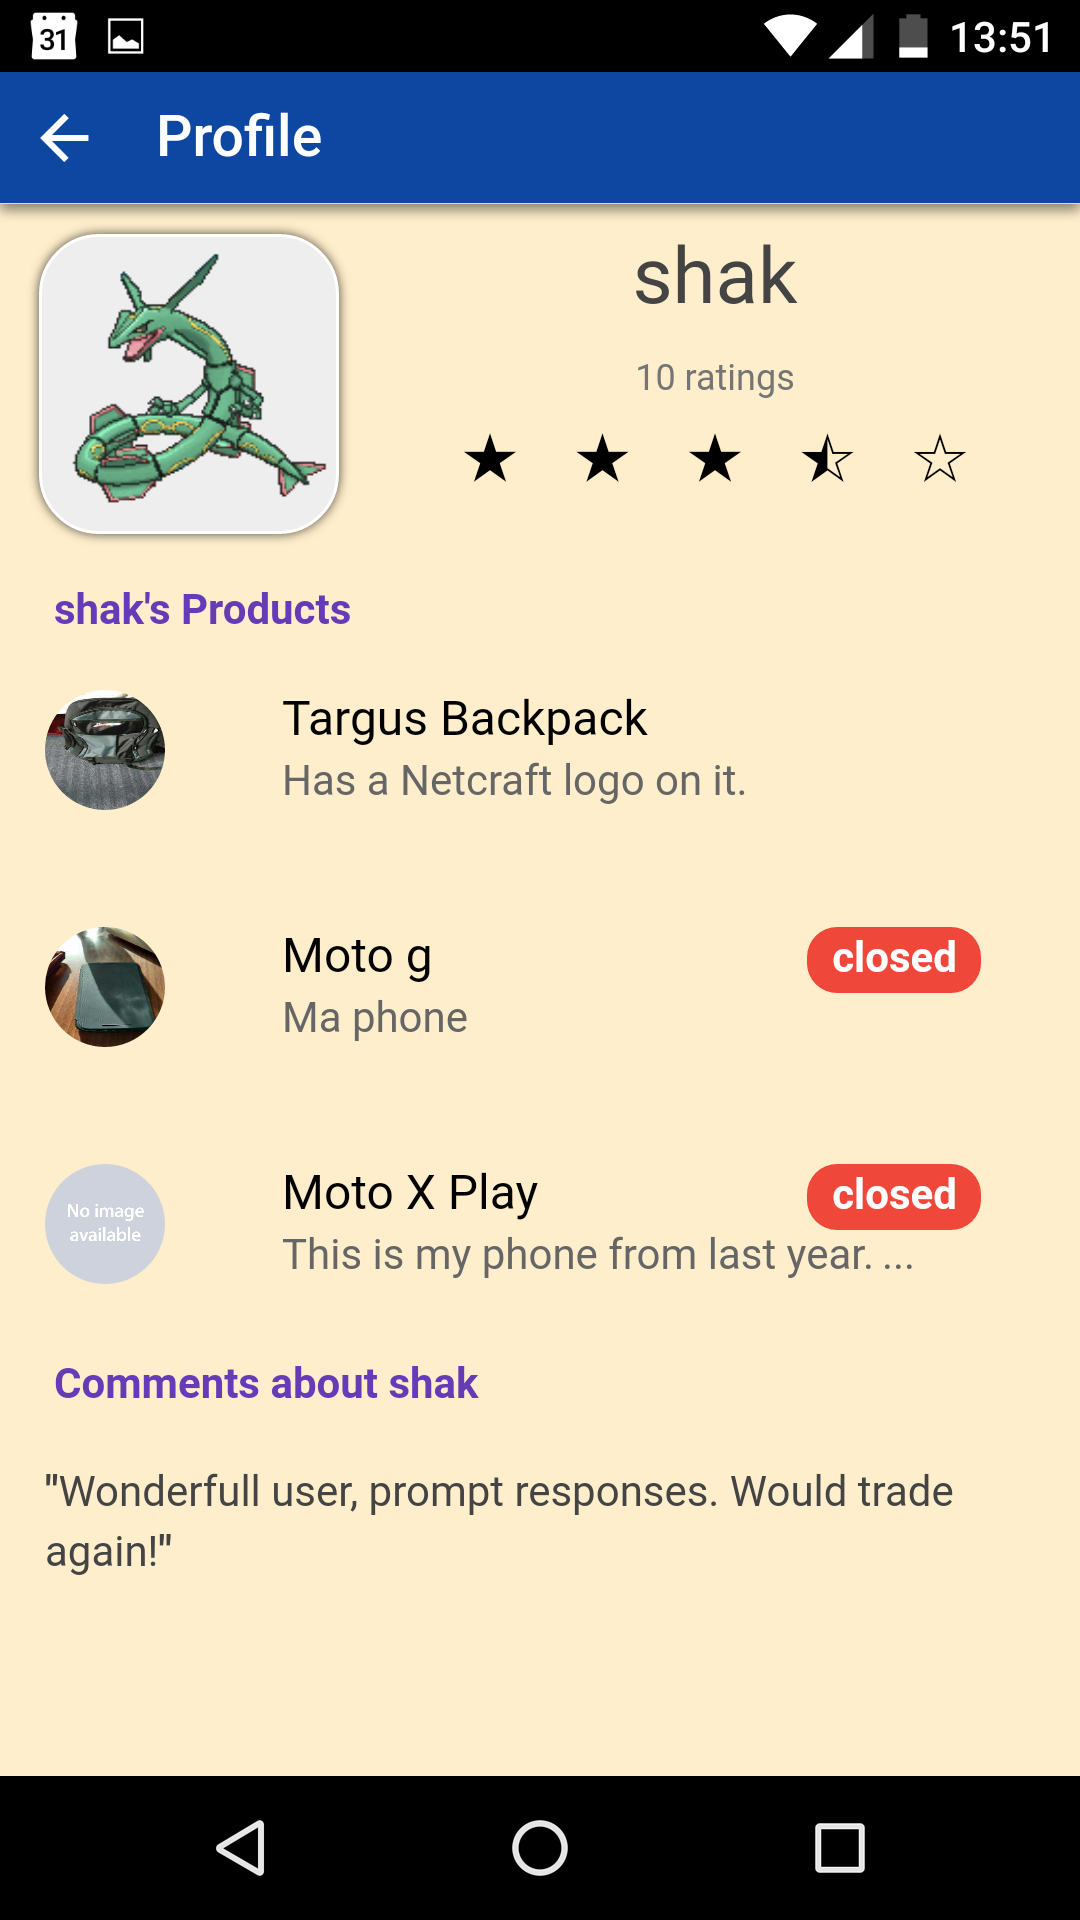
\includegraphics[width=\textwidth]{profile}
        \caption{Profile}
        \label{fig:profile}
    \end{subfigure}
    ~
    \begin{subfigure}[b]{0.3\textwidth}
        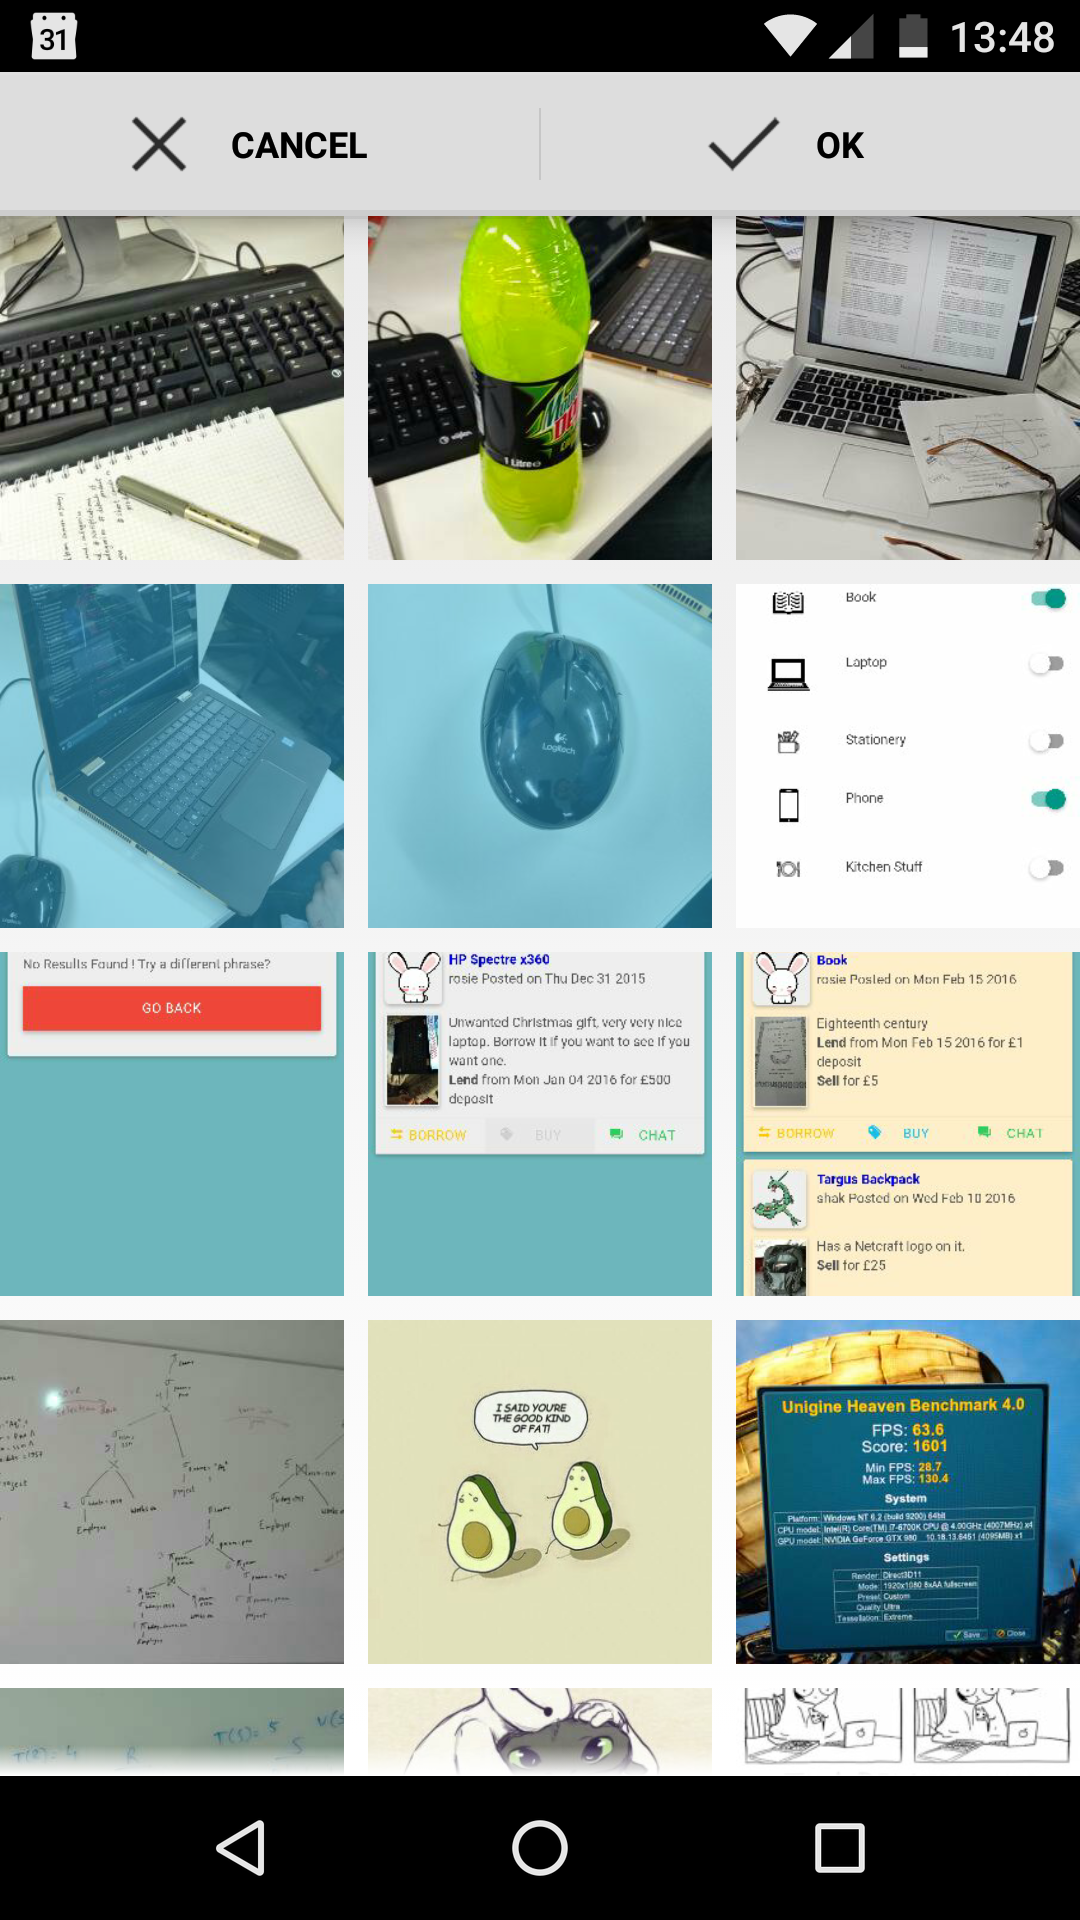
\includegraphics[width=\textwidth]{gallery-select}
        \caption{Gallery Select}
        \label{fig:gallery-select}
    \end{subfigure}
    ~
    \begin{subfigure}[b]{0.3\textwidth}
        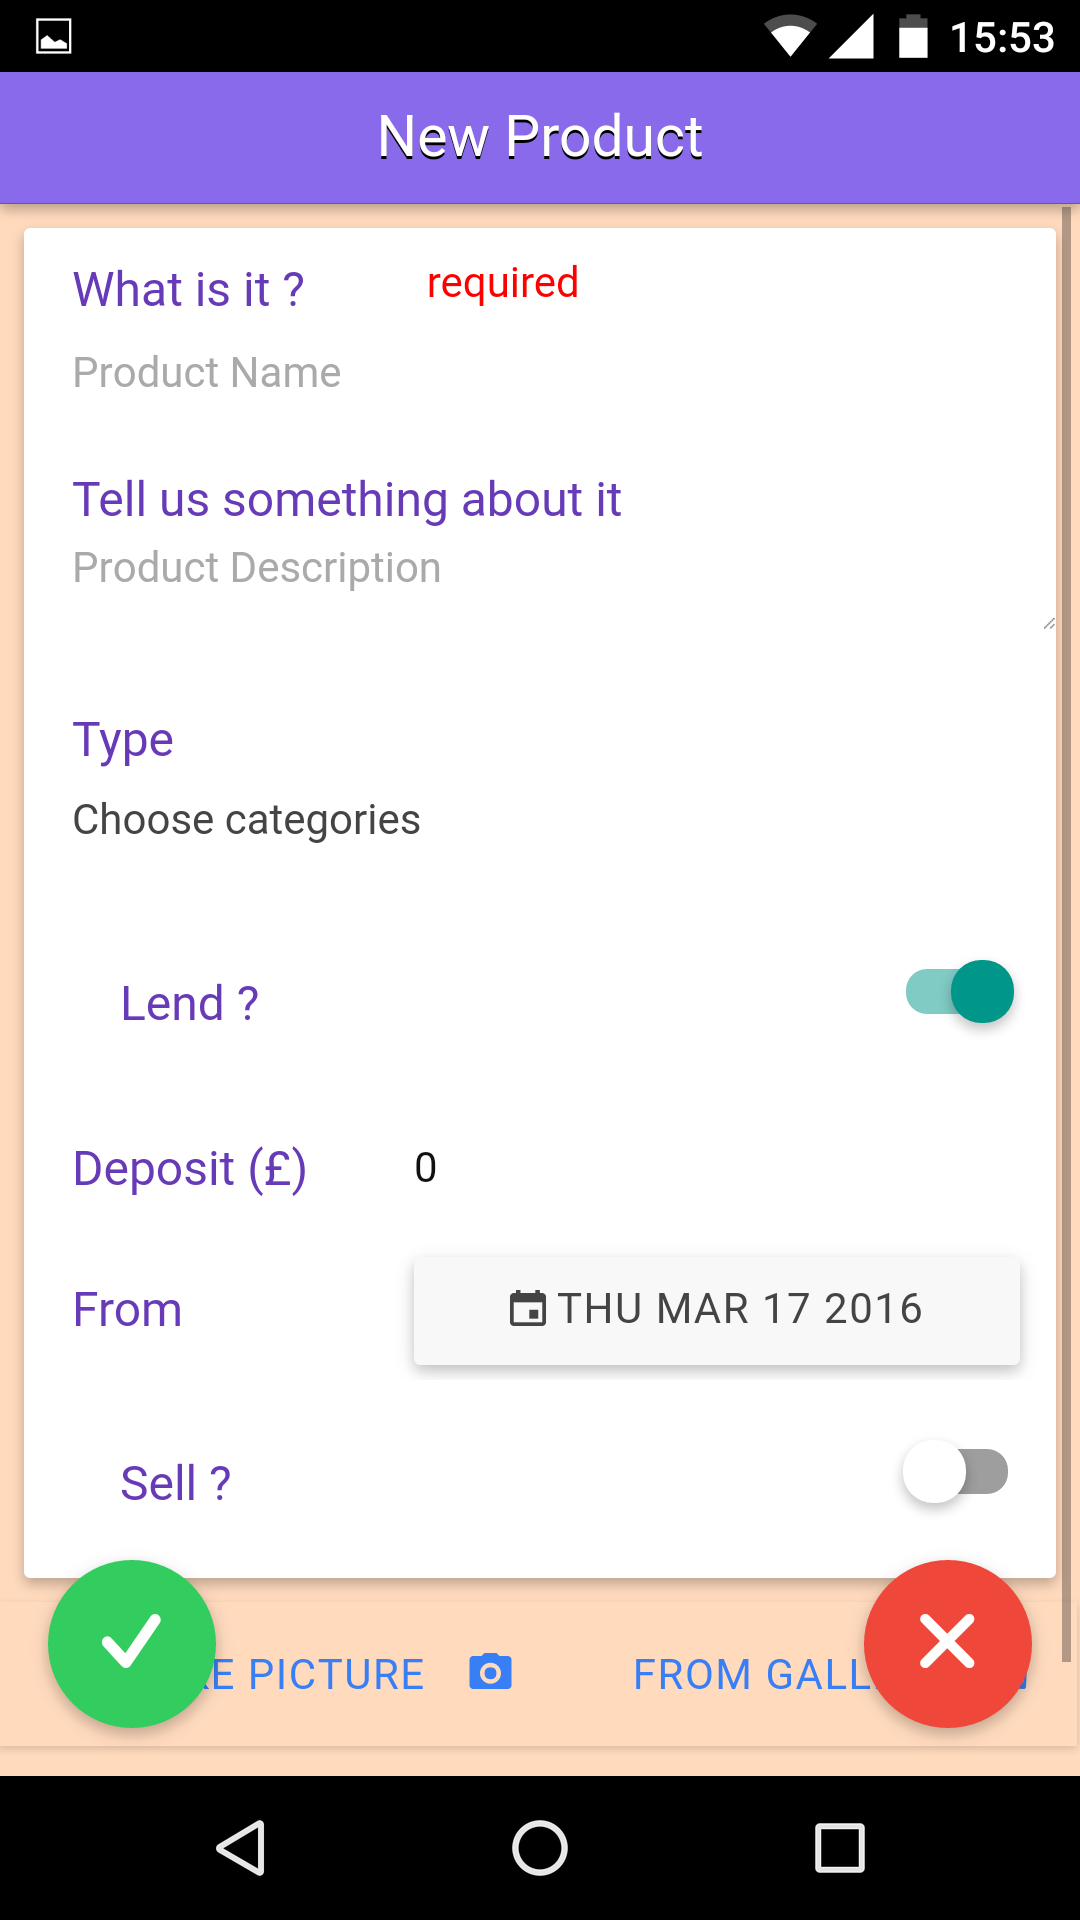
\includegraphics[width=\textwidth]{add}
        \caption{Add Product}
        \label{fig:add}
    \end{subfigure}
    ~
    \begin{subfigure}[b]{0.3\textwidth}
        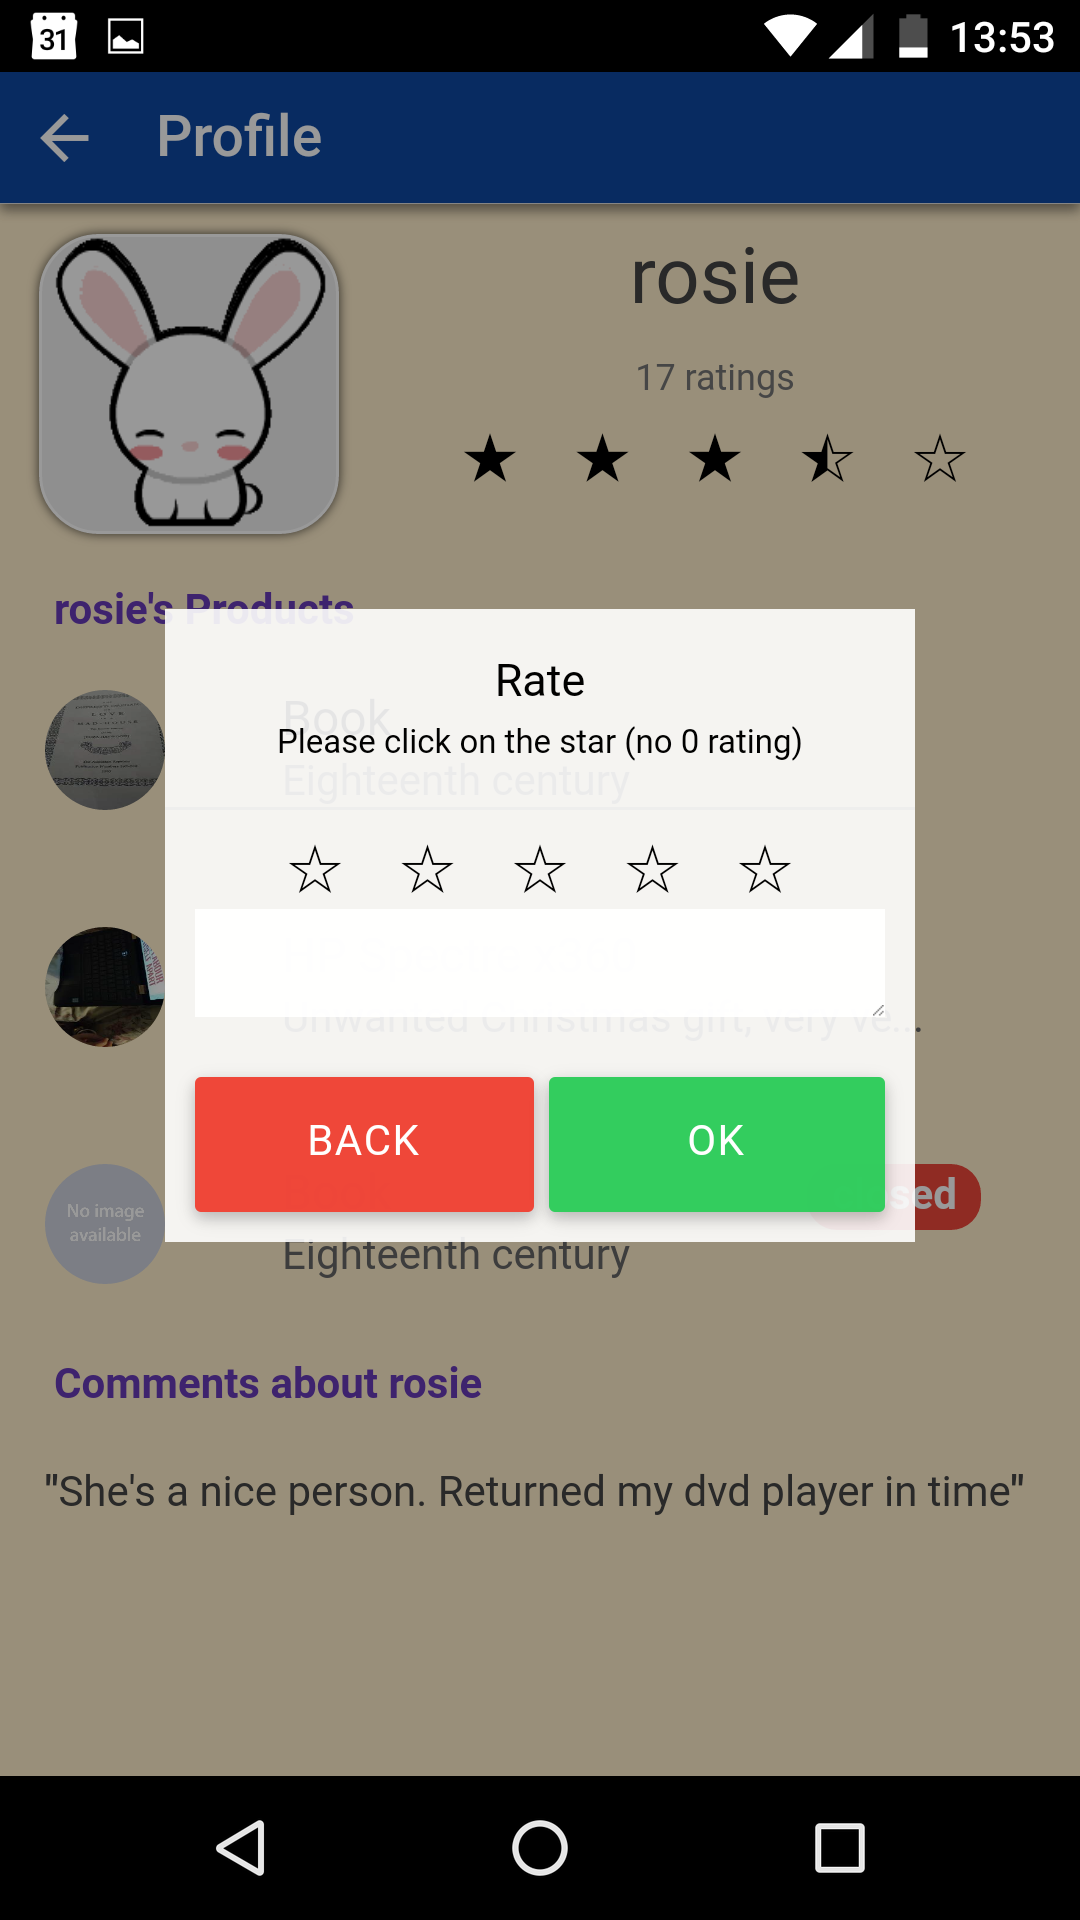
\includegraphics[width=\textwidth]{rate}
        \caption{Rate}
        \label{fig:rate}
    \end{subfigure}
    ~
    \begin{subfigure}[b]{0.3\textwidth}
        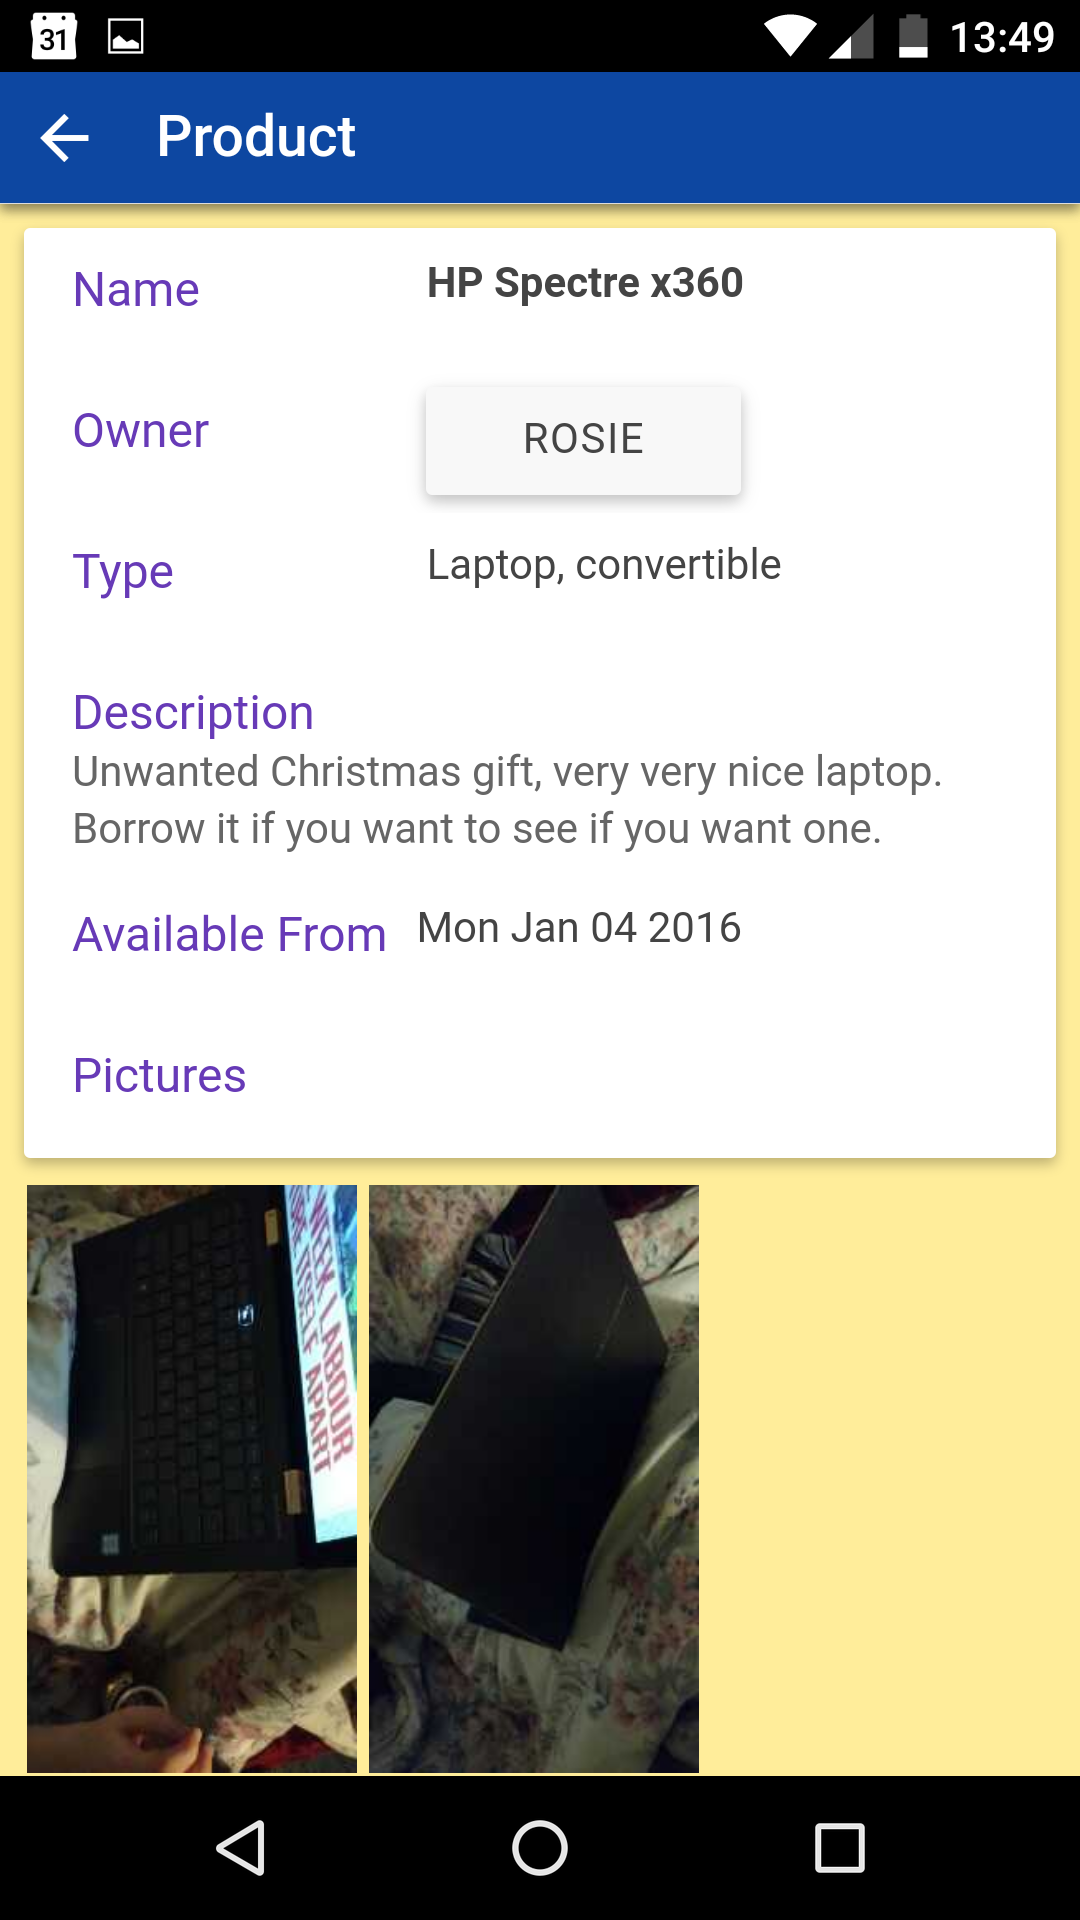
\includegraphics[width=\textwidth]{product}
        \caption{Product Detail}
        \label{fig:product}
    \end{subfigure}
    ~
    \begin{subfigure}[b]{0.3\textwidth}
        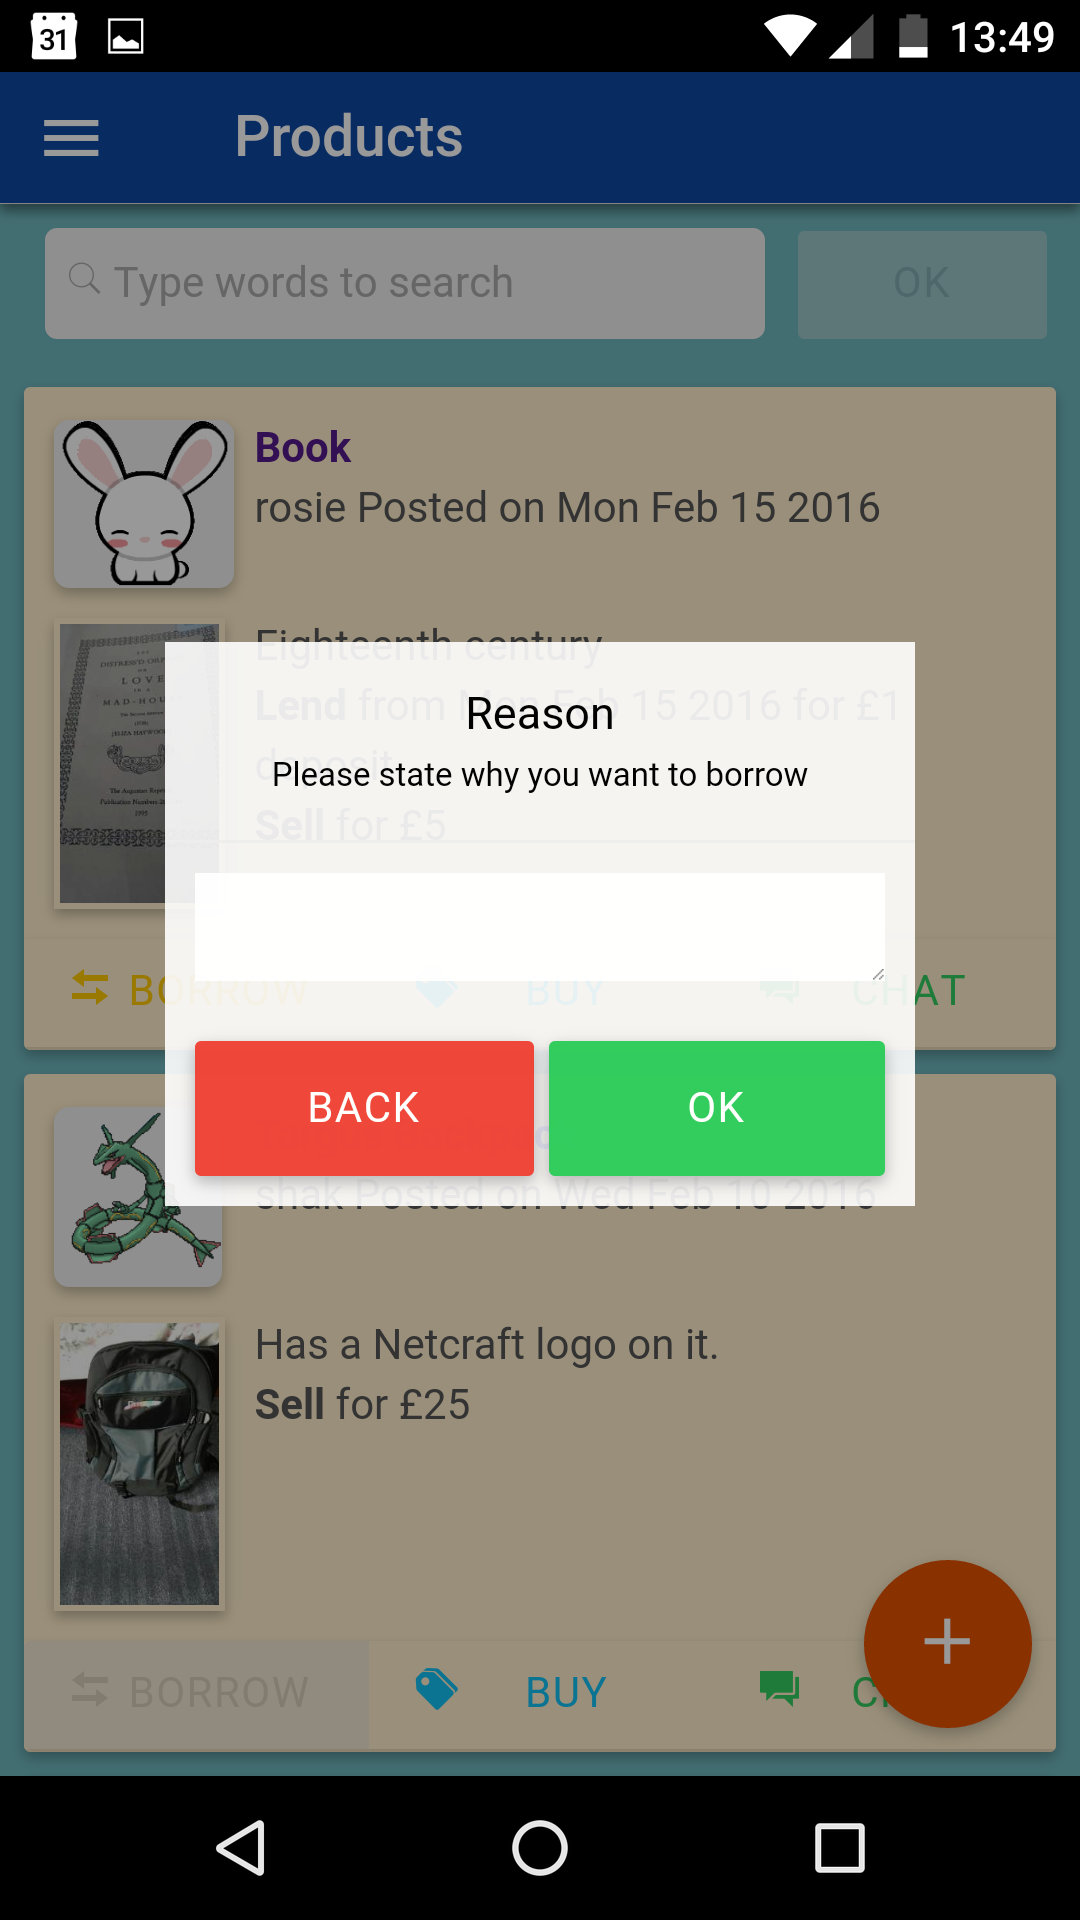
\includegraphics[width=\textwidth]{lend}
        \caption{Borrow}
        \label{fig:lend}
    \end{subfigure}
    ~
    \begin{subfigure}[b]{0.3\textwidth}
        
\includegraphics[width=\textwidth]{product-offer}
        \caption{Requests}
        \label{fig:requests}
    \end{subfigure}
    \caption{Screenshots}\label{fig:scr4}
\end{figure}
\chapter{Project Organisation}
\label{chap:proj-org}
In this chapter, I have discussed the overall project plan and the organisation in various stages in detail.

\section{Plan Overview}

The overall plan for the project was to - start with some simple assumptions and make a simple prototype, gather user stories through interviews, develop in four sprints, perform UX evaluation and finish development (Appendix \ref{appendix:gantt}). I used Microsoft Visual Studio online to keep track of the user stories (backlog), a physical kanban board for bugs, Gantt chart for the general plan, Github for version control and Mendeley for formal background research. The project was to be completed between October and March.

\section{Initial Sprint}

I started the first sprint in early October with a goal of producing a very simple client app, working together with a simple server and database. The initial user stories were based on the following assumptions and put into the first iteration of product backlog, seen in Figure \ref{fig:backlog-v1} - 

\begin{itemize}
	\item There will be a number of users and things.
	\item Most routes will require user authentication.
	\item Documentation should be adequate for future development.
\end{itemize}

This prototype was then used in a set of user interviews to elicit more requirements and form user stories.

\begin{figure}[!h]
    \centering
    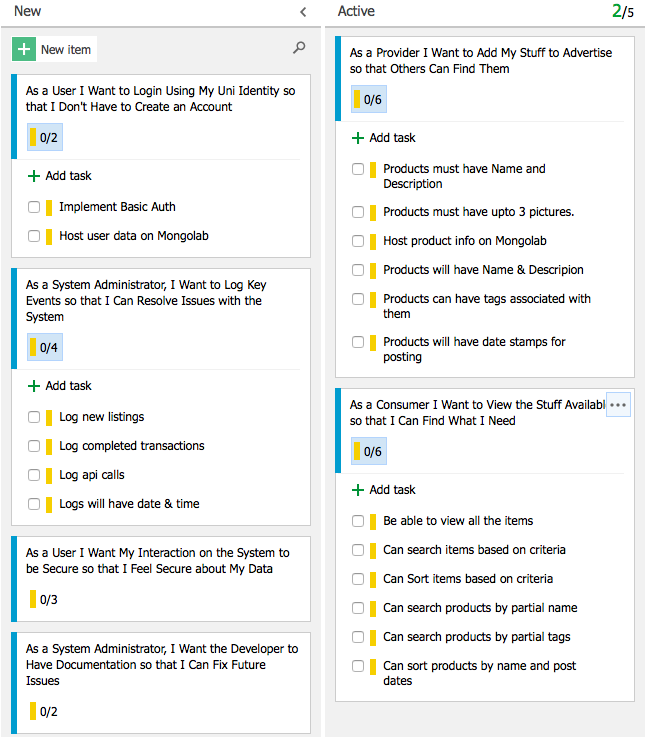
\includegraphics[height = \textwidth, width=\textwidth, keepaspectratio]{backlog_v1}
    \caption{Backlog v1}\label{fig:backlog-v1}
\end{figure}

\section{RE with User Participation}

As planned, I set up interviews with 5 potential users, all UoS students. \textit{Participatory Design} is to invite end users in the designing process of software development. Chapter \ref{chap:user} describes the process and my experiences in detail. In short, my target was to ask the interviewees some open ended questions that will help me better understand their \textit{pain points} and have them draw some wireframes on paper. I used the information gathered to include new user stories and select work for the second sprint.

\section{Intermediate Sprints}

The next stage was to develop the user stories from the updated product backlog (Figure \ref{fig:backlog-v2}) in three sprints. After each sprint, I spent 3-4 days in review to test the \textit{user stories} (\textit{not} development testing) to decide if they can be considered closed (\textit{acceptance criteria}, usually performed by the product owner), updated with more work, be simplified etc. I also recorded the bugs, separate on a physical kanban board.\\

At that point, I also re-prioritised the backlog, so that I could complete the user stories that can have the most effect with the least effort (\textit{impact vs feasibility}). I used both the user interviews and my abilities in required technologies as metrics for this procedure.

\subsection{Sprint 2}

This sprint's targets were as follows - 

\begin{itemize}
	\item A basic user profile functionality.
	\item Adding products, view list of added products and basic search.
	\item Simple logging for each HTTP request.
\end{itemize}

The review was shorter than planned, as the prototype was still quite simple. The updated product backlog can be seen in Figure \ref{fig:backlog-v3}. It introduced a new column - \textit{Disregarded} where I placed the user stories that would not be included in the final version. A progress report was submitted after this sprint.

\begin{figure}[!h]
    \centering
    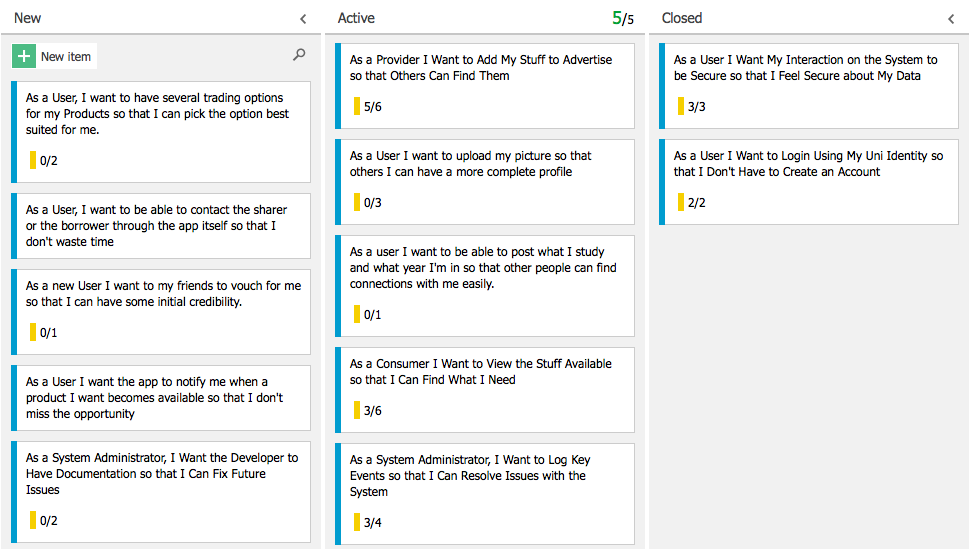
\includegraphics[height = \textwidth, width=\textwidth, keepaspectratio]{backlog_v2}
    \caption{Backlog v2}\label{fig:backlog-v2}
\end{figure}

\subsection{Sprint 3}

The next sprint, performed during the Christmas period, was set to complete user stories regarding - 

\begin{itemize}
	\item Adding some trading options - lend, sell etc.
	\item Allow offers/requests to be made regarding products.
	\item Allow users to accept/decline offers.
\end{itemize}

Another major goal in this iteration was to start formal JavaScript testing, starting from server routes. I discuss about testing in more detail in Chapter \ref{chap:test}. This sprint review revealed two choices for the next sprint - 

\begin{description}
	\item [Chat] functionality between two users.
	\item [Push Notifications] sent regarding offers made on products.
\end{description}

Whereas, every user wanted push notifications for not only offers, but also for several other user stories, chatting only serves a single user story - \textit{in-app communication}. Each required a significant learning curve, and project plan and timings could only accommodate one to be done \textit{well}. I chose notifications, because it could be used in various purposes and allow me to gain better insights into mobile development (\textit{push notifications} being more prevalent on mobile platforms). The updated product backlog can be seen in Figure \ref{fig:backlog-v4}.

\begin{figure}[!h]
    \centering
    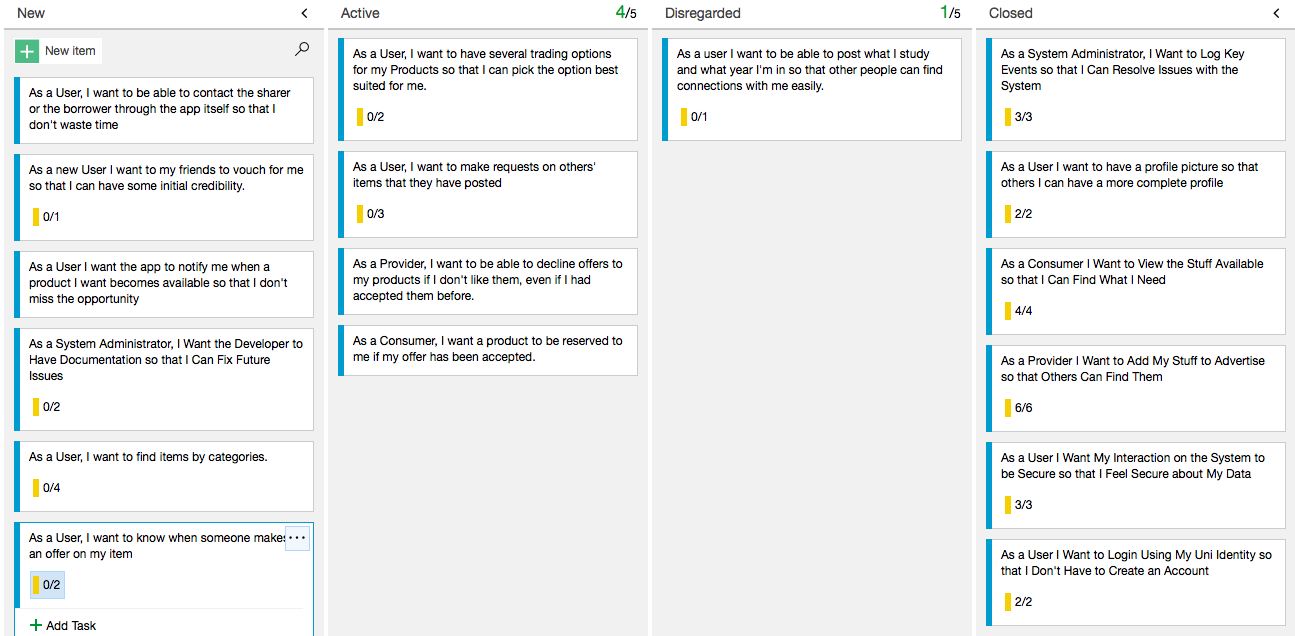
\includegraphics[height = \textwidth, width=\textwidth, keepaspectratio]{backlog_v3}
    \caption{Backlog v3}\label{fig:backlog-v3}
\end{figure}

\subsection{Sprint 4}

As planned, this iteration, starting in the Semester 2, was to finish the user stories already present on the backlog. The primary goal in this iteration was to implement push notifications regarding the offers made on products. Some of the major tasks were - 

\begin{itemize}
	\item Integrate GCM with the server.
	\item Register client device for push notifications.
	\item Send push notifications to the correct users, in time.
\end{itemize}

During the development and review, I realised that push notifications were both unreliable and quite difficult to test. However, I marked the user stories as done by simplifying the acceptance criteria. The next stage was to perform User Experience (UX) evaluation on the current prototype.

\begin{figure}[!h]
    \centering
    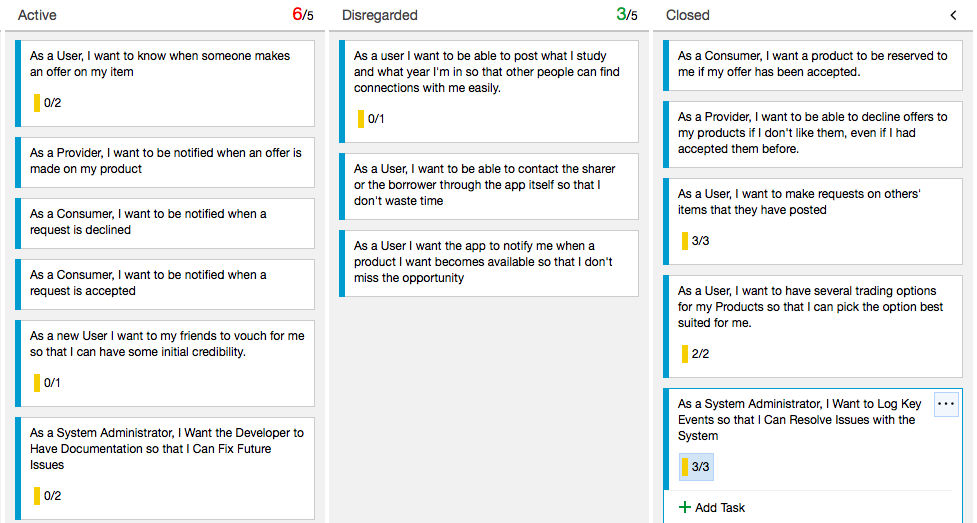
\includegraphics[height = \textwidth, width=\textwidth, keepaspectratio]{backlog_v4}
    \caption{Backlog v4}\label{fig:backlog-v4}
\end{figure}

\begin{figure}[!h]
    \centering
    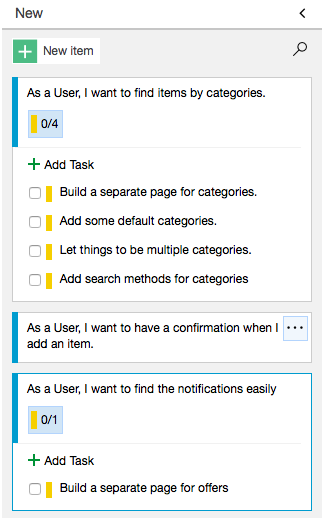
\includegraphics[height = 0.8\textwidth, width=\textwidth, keepaspectratio]{backlog_v5}
    \caption{Final User Stories}\label{fig:backlog-v5}
\end{figure}

\section{UX Evaluation}

Interviews were set up with the same users who were interviewed earlier to evaluate the prototype. I have discussed the process in detail in chapter \ref{chap:user}. The results were largely satisfactory. However, it also gave rise to a number of issues, found in Appendix \ref{appendix:ux}. I evaluated the issues and prioritised them based on effort needed to address them. The final backlog was updated as seen in Figure \ref{fig:backlog-v5}.

\section{Final Sprint}

The final sprint's goal was to resolve most of the simple issues found in the UX evaluation and focus on at least half of the major issues. The results included - 

\begin{itemize}
	\item New app layout to utilise white space better.
	\item Separate sections for categories and offer notifications.
\end{itemize}

In the final sprint review, I found most of my originally planned specifications to be completed to a satisfactory level (for an alpha stage prototype, not a production ready app). So, I discarded the final UX evaluation interviews, which were only planned if significant issues were found in the previous evaluation.


%% This chapter discusses the technologies and the architecture
\chapter{Architecture \& Technology Overview}

In this chapter, I will briefly discuss the frameworks used in the project, followed by how well they served their intended purpose as well as how they work in tandem as a complete system.

%%%%%%%%%%%%%%%%%%%%%%%%%%%%%%%%%%%%%%%%%%%%%%%%%%%%%%%%
%% List the tehnologies that were used.
\section{Technologies Used}

\textbf{JavaScript} is the base programming language in the project. However, each part of the system is built using a suitable framework. In this section, I will only list the frameworks.

\subsection{Client Application}

\textbf{Ionic} \cite{ionic-site} is used as the 'app' framework. It provides the GUI components as HTML and CSS and plug-ins for platform specific support for mobile  features like camera, calendar etc. from \textbf{Cordova} \cite{ngcordova-site}. As for the JavaScript part of the application, it uses an opinionated framework, \textbf{AngularJS} \cite{angular-site}, to provide interactivity and navigation.

\subsection{Server Application}

I used \textbf{NodeJS} \cite{nodejs-site}, a non-blocking JavaScript runtime, and \textbf{Express} \cite{expressjs-site}, an unopinionated framework, to build the server. \textbf{MongoDB} \cite{mongodb-site}, a NoSQL database, was used for storage.

\subsection{Test Suits}

\textbf{MochaJS} \cite{mocha-site}, a JavaScript test framework, was used as the automated test runner and the assertion library was \textbf{ShouldJS} \cite{shouldjs-site}.

\subsection{Cloud Platform}

The server was hosted on \textbf{Heroku} \cite{heroku-site}, a PaaS (Platform-as-a-Service), while \textbf{mLab} \cite{mlab-site} hosted the database.

%%%%%%%%%%%%%%%%%%%%%%%%%%%%%%%%%%%%%%%%%%%%%%%%%%%%%%%%


%%%%%%%%%%%%%%%%%%%%%%%%%%%%%%%%%%%%%%%%%%%%%%%%%%%%%%%%
%% How well did these perform from expected
\section{Applicability of Technology}

In this section, I will discuss how the aforementioned frameworks helped in development.

\subsection{Ionic \& AngularJS}

Ionic provides HTML 5 and CSS built components like in Figure \ref{fig:ionic-comp-ex}. These are easily customisable and provides great usability on mobiles. Using the CLI (Command Line Interface), I easily added plug-ins  (\texttt{ionic add <plugin>}), different platform support (\texttt{ionic add <platform>}) and generated platform specific installable app (\texttt{ionic <build || run> <platform>}) without writing any native code.\\

\begin{figure}[h]
    \centering
    \begin{subfigure}[b]{0.3\textwidth}
        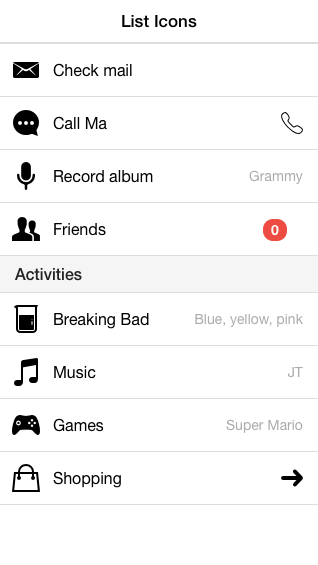
\includegraphics[width=\textwidth]{ionic-a}
    \end{subfigure}
    ~
    \begin{subfigure}[b]{0.3\textwidth}
        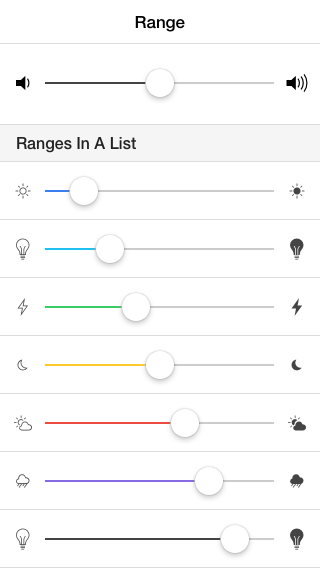
\includegraphics[width=\textwidth]{ionic-b}
    \end{subfigure}
    ~ 
    \begin{subfigure}[b]{0.3\textwidth}
        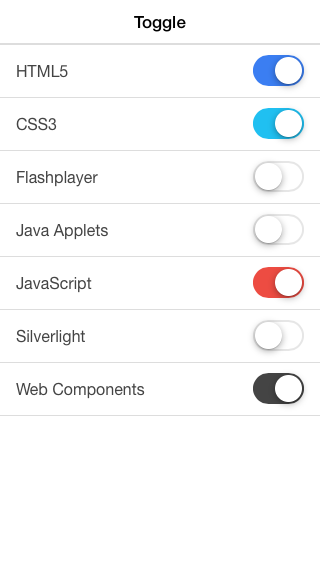
\includegraphics[width=\textwidth]{ionic-c}
    \end{subfigure}
    \caption{Ionic Component Examples}\label{fig:ionic-comp-ex}
\end{figure}

I structured the code in MVC (Model View Controller) pattern and created navigation between views using AngularJS. Angular's \textit{directives} bind a view with the underlying data structure, for example - bind a table to a list, so updating views is made very easy.

\subsection{NodeJS \& MongoDB}

NodeJS is completely asynchronous, so it can utilise IO operations (database query) very efficiently (compared to Apache for example) and serve magnitudes of more clients (Figure \ref{fig:node-comp-ex} \cite{tomislav-site}), despite being single-threaded. In fact, it is 2.5 magnitudes faster than PHP and cpu-memory efficient. As the system is meant to handle many users simultaneously, it is highly advised to use Node to handle such real-time communication, specially in tandem with hybrid platforms \cite{Chaniotis:2015}.\\

\begin{figure}[h]
    \centering
    \begin{subfigure}[b]{0.45\textwidth}
        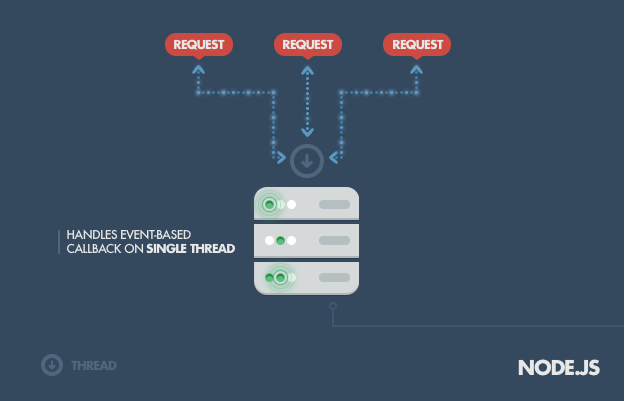
\includegraphics[width=\textwidth]{node-a}
    \end{subfigure}
    ~
    \begin{subfigure}[b]{0.45\textwidth}
        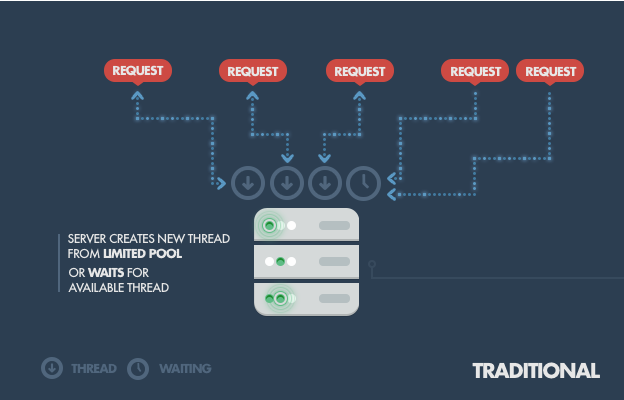
\includegraphics[width=\textwidth]{node-b}
    \end{subfigure}
    \caption{NodeJS}\label{fig:node-comp-ex}
\end{figure}

MongoDB is schema-less and document driven. As a NoSQL database, it is highly scalable and can handle unstructured data, multimedia and social-media content efficiently \cite{cornelia:2015}. Indeed, Mongo's flexibility was necessary for fast prototyping and suitable for the app's intention.

\subsection{Heroku \& mLab}

Out of the well known PaaS such as Bluemix \cite{bluemix-site}, Openshift \cite{openshift-site}, AppEngine \cite{gae-site} etc., Heroku is by far the easiest to use (to get started and deploy), in my opinion, and has the best community support. A PaaS takes care of infrastructure tasks like hosting a server, scaling it etc. So, I could focus more on development. As for mLab, it is a generic MongoDB hosting site with free usage upto 500 MB and easily integrated with Heroku.

\subsection{Issues}
\label{subsec:issues}

There were some issues that could not be avoided with the selection of technology - 

\begin{description}

	\item [GCM] (Google Cloud Messaging) \cite{gcm-site} is the only entity that can send push notification to an Android phone (even though intermediate frameworks, e.g. Ionic Push, can be involved). While it is possible to verify if a request for notification has been accepted, when it gets delivered cannot be controlled in any way. Often a notification will be found as sent, but it will not actually arrive for hours. The probable reason is that, I used a \textit{free} GCM service rather than a \textit{paid} one.
	
	\item [Base64] images \cite{base64-site} are ASCII encodings of binary image files. Although, Amazon S3 \cite{s3-site} is the preferred service to store images, it is not free. So, I stored images as very large strings in MongoDB. This should be avoided a production-ready app.
	
\end{description}

%%%%%%%%%%%%%%%%%%%%%%%%%%%%%%%%%%%%%%%%%%%%%%%%%%%%%%%%


%%%%%%%%%%%%%%%%%%%%%%%%%%%%%%%%%%%%%%%%%%%%%%%%%%%%%%%%
%% Discuss how the technologies work together
\section{Architecture}

%%%%%%%%%%%%%%%%%%%%%%%%%%%%%%%%%%%%%%%%%%%%%%%%%%%%%%%%

In this section I will discuss how different parts of the project comes together. Figure \ref{fig:archi} is the complete architecture diagram which will be referred to in the following sections.

\begin{figure}[h]
    \centering
    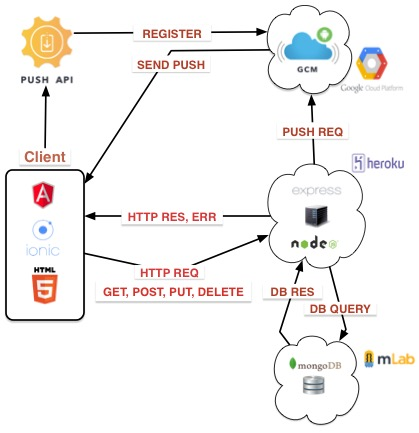
\includegraphics[height=0.7\textwidth]{architecture}
    \caption{System Architecture}\label{fig:archi}
\end{figure}

\subsection{Client-Server Communication}

The Ionic client app makes requests to the NodeJS server on Heroku to retrieve/create/update/delete various data artefacts. These requests are authorised by the \textit{PassportJS Local Strategy} (by unique username-password, rather than a social network). The server then asynchronously handles each request.

\subsection{Server-Databse Communication}

The server contacts the MongoDB database on mLab asynchronously (for which it has a key) for each client request. After the results reach the server, it asynchronously passes them to the Client. The client thus never directly contacts the database.

\subsection{Push Notification}

When the app is opened on a mobile first time, Client sends a GCM registration request via the Ionic Push API. This API registers the app, sends back a token to the client. Finally, the client sends the token to the server and it, in turn, saves it on mLab. In future, an event may be triggered on the server (e.g. new offer from a user) which may require a push notification to one-or-more clients. It sends a request to the GCM server to send a notification to the given tokens. GCM takes care of the actual sending of the notification.
\chapter{Implementation}
In this chapter, I will explain in detail, how the different parts of the project were designed and built.

%%%%%%%%%%%%%%%%%%%%%%%%%%%%%%%%%%%%%%%%%%%%%%%%%%%%%%%%%%%%%%%%%%%%%%%%%%%%
%% explain the data models
%%
%%%%%%%%%%%%%%%%%%%%%%%%%%%%%%%%%%%%%%%%%%%%%%%%%%%%%%%%%%%%%%%%%%%%%%%%%%%%
\section{Data Models}

The system needs to handle data regarding - 

\begin{itemize}
	\item \textit{People} who will use the system.
	\item Details of \textit{Something} that can be traded, lent, rented or sold etc.
	\item Record of \textit{interaction} between people regarding some item of interest.	
\end{itemize}

Data models were designed keeping these in mind. The models were developed as they were needed for user stories during a sprint.

%%%%%%%%%%%%%%%%%%%%%%%%%%%
%% Model defs
%%
%%%%%%%%%%%%%%%%%%%%%%%%%%%
\subsection{Model Definitions}

\begin{description}
	\item [User] : Users must have a unique username and a password (hashed). They can also have a default avatar (as Base64 or URI) and an initial rating of 0. Rating is primitive and only accounts for the average.
	\item [PushToken] : Every User must have a PushToken object reference. These objects contain the device tokens generated by GCM by push registration.
\end{description}

%% user data model diagram
\begin{figure}[!h]
\centering

\begin{tikzpicture}

\umlclass[x=0, y=0]{User}{
  \textbf{* username} : \texttt{String} \\
  \textbf{* password} : \texttt{String}\\
  \textbf{\_pushTokens} : \texttt{PushToken.\_id}\\
  \textbf{avatar} : \texttt{String}\\
  \textbf{rating} : \texttt{\{ count : Number, average: Number \}}\\
}{}

\umlclass[x=8, y=0]{PushToken}{
  \textbf{* \_user} : \texttt{User.\_id} \\
  \textbf{tokens} : \texttt{[String]}\\
}{}

\end{tikzpicture}
\caption{User Model} \label{fig:user-model}
\end{figure}

\begin{description}
	\item [Thing] : A Thing is an abstraction for either a service or an object. It must have a name and an owner. Other fields include name, description and type (category). \texttt{closed} records whether the item can be acquired or not, whereas \texttt{\_reservedTo} is the User whose offer for the thing was last accepted.
	\item [Lend] : A Lend object is created when a User wants others to borrow a Thing (which gets a reference to that object).
\end{description}

%% Thing data model diagram
\begin{figure}[!h]
\centering
\begin{tikzpicture}

\umlclass[x=0, y=0]{Thing}{
  \textbf{* name} : \texttt{String} \\
  \textbf{type} : \texttt{String}, \\
  \textbf{desc}: \texttt{String}, \\
  \textbf{* \_owner} : \texttt{User.\_id}\\
  \textbf{pictures} : \texttt{[String]}\\
  \textbf{\_lend} : \texttt{Lend.\_id}\\
  \textbf{\_sell} : \texttt{Sell.\_id}\\
  \textbf{\_reservedTo} : \texttt{Offer.\_id}\\
  \textbf{closed} : \texttt{Boolean}\\
}{}

\umlclass[x=6, y=0.5]{Offer}{
  \textbf{* \_from} : \texttt{User.\_id} \\
  \textbf{* \_to} : \texttt{User.\_id}, \\
  \textbf{* \_borrow}: \texttt{Lend.\_id}, \\
  \textbf{* \_buy} : \texttt{Sell.\_id}\\
  \textbf{reason} : \texttt{String}\\
  \textbf{accepted} : \texttt{Boolean}\\
  \textbf{declined} : \texttt{Boolean}
}{}

\umlclass[x=0, y=-5]{Sell}{
  \textbf{* \_thing} : \texttt{Thing.\_id} \\
  \textbf{price} : \texttt{Number}
}{}

\umlclass[x=6, y=-4.5]{Lend}{
  \textbf{* \_thing} : \texttt{Thing.\_id} \\
  \textbf{deposit} : \texttt{Number}, \\
  \textbf{from}: \texttt{Date}, \\
  \textbf{to} : \texttt{Date}\\
}{}

\end{tikzpicture}
\caption{Thing Model} \label{fig:thing-model}
\end{figure}

\begin{description}
	\item [Sell] : Similar to Lend, it only gets created when a User wants others to buy a Thing. A Thing can have both \texttt{\_sell} and \texttt{\_lend}.
	\item [Offer] : An Offer is created when a User wants to buy/borrow (depending on which options are available) some item for some \textit{reason}. It can be accepted or declined (both initially set to false).
\end{description}

\subsection{Model Design Choices}

Things can be \textit{closed}, rather than removed from the system once a transaction takes place, so that, a borrowed item could be made \textit{active} once it has been returned, rather than posting again.\\

Offers have both \textit{accepted} and \textit{declined} fields, rather than a toggle, because, the initial condition, where it is neither accepted nor declined, can be interpreted.\\

Images, as explained in Section \ref{subsec:issues}, are saved directly as Strings, rather than BLOBs (Binary Large OBject) because of database free account restriction.\\

User objects do not directly have access to device tokens, so that, unused or invalid tokens can be destroyed in future without manipulating the main User object.\\

Lend or Sell options are whole objects, rather than a field on a Thing, because, an Offer should be distinguished between a borrow or a buy offer. Rather than creating an Offer hierarchy, these intermediate objects are referenced in respective Offer-Thing combos.

\section{Server}

In this section, I will discuss how the RESTful API was created, database and GCM integration was done and how authentication is performed.

\subsection{Routes}

\href{https://en.wikipedia.org/wiki/Representational_state_transfer}{REST} (Representational State Transfer) is the software architectural style of WWW (World Wide Web) \cite{Fielding:2000}. Simply put, a client makes requests, usually HTTP (Hypertext Transfer Protocol) requests, at specific routes. The methods are usually CRUD (Create Read Update Delete).\\

This server was then hosted on heroku at \href{http://project-api.herokuapp.com/}{http://project-api.herokuapp.com/}. Each route is superseded by \texttt{/api} to denote a version number for the api. Table \ref{table:user-routes}, \ref{table:thing-routes} and \ref{table:offers-routes} respectively shows routes for User, Thing and Offer objects. These routes were created with the following in mind -

\begin{itemize}
	\item Users will need to add new items, retrieve all or searched items.
	\item The things will be updated, requested upon and eventually closed.
	\item Users will want to request for items, respond to requests and rate others.
\end{itemize}

\newcommand{\NA}{---}

\begin{table}[!h]
    \centering
    \begin{tabularx}{\textwidth}{lcXcc}
    \toprule
    \centering
    \emph{\textbf{Route}} \texttt{/users} & \emph{\textbf{Method}} & \emph{\textbf{Use}} & \emph{\textbf{Params}} & \emph{\textbf{Returns}} \\
    \midrule
    \texttt{/}
    		& \texttt{GET} & get all the \newline users on the system  & \NA 			 & \texttt{[User]} \\ \cline{2-5} \noalign{\smallskip}
    		& \texttt{POST} & create a new user on the system  & \texttt{User}  & \texttt{User}    \\ 
    \midrule
    \texttt{/:uname} 
    		& \texttt{GET} & get a particular user & \NA & \texttt{User}  \\ \cline{2-5} \noalign{\smallskip}
    		& \texttt{PUT} & update a single user & \texttt{User} & \texttt{User} \\
    	\midrule
    \texttt{/:uname/things}
    		& \texttt{GET} & get all the things for a user & \NA & \texttt{[Thing]} \\ \cline{1-5} \noalign{\smallskip}
    \texttt{/:uname/rating}
    		& \texttt{PUT} & rate a user & \texttt{[User.rating]} & \NA  \\ \cline{1-5} \noalign{\smallskip}
	\texttt{/offers/to}
		& \texttt{GET} & get all the offers made to a user & \NA & \texttt{[Offer]}  \\
    \bottomrule
    \hline
    \end{tabularx}
    \caption{User Routes}
    \label{table:user-routes}
\end{table}

\begin{table}[!h]
    \centering
    \begin{tabularx}{\textwidth}{lcXcc}
    \toprule
    \centering
    \emph{\textbf{Route}} & & & \\
    \texttt{/things} & \emph{\textbf{Method}} & \emph{\textbf{Use}} & \emph{\textbf{Params}} & \emph{\textbf{Returns}} \\
    \midrule
    \texttt{/}
    		& \texttt{GET} & get all the things on system  & \NA 			& \texttt{[Thing]} \\ \cline{2-5} \noalign{\smallskip}
    		& \texttt{POST} & create a new thing on system & \texttt{Thing} & \texttt{Thing} \\
	\midrule    	
    	\texttt{/:id}
    		& \texttt{GET} & get a particular thing & \NA & \texttt{Thing} \\ \cline{2-5} \noalign{\smallskip}
    		& \texttt{PUT} & update a single thing & \texttt{Thing} & \texttt{Thing} \\ \cline{2-5} \noalign{\smallskip}
    		& \texttt{DELETE} & delete a single thing & \NA & \texttt{Thing} \\
    	\midrule
    	\texttt{/:id/close}
    		& \texttt{POST} & close a single thing & \NA & \texttt{Thing} \\
    \bottomrule
    \hline
    \end{tabularx}
    \caption{Thing Routes}
    \label{table:thing-routes}
\end{table}

\begin{table}[!h]
    \centering
    \begin{tabularx}{\textwidth}{lcXcc}
    \toprule
    \centering
    \emph{\textbf{Route}} & & & \\
    \texttt{/things/:id/offers} & \emph{\textbf{Method}} & \emph{\textbf{Use}} & \emph{\textbf{Params}} & \emph{\textbf{Returns}}\\
    \midrule
    \texttt{/:offer\_id}
    		& \texttt{GET} & get all offers for a thing & \NA & \texttt{[Thing]} \\ \cline{1-5} \noalign{\smallskip}
    	\texttt{/:offer\_id/accept}
    		& \texttt{GET} & accept an offer & \NA & \texttt{Thing} \\ \cline{1-5} \noalign{\smallskip}
    	\texttt{/:offer\_id/decline}
    		& \texttt{POST} & decline an offer & \NA & \texttt{Thing} \\
    \bottomrule
    \hline
    \end{tabularx}
    \caption{Offers Routes}
    \label{table:offers-routes}
\end{table}

\subsection{Code Structure}

There are 3 main sections in this server :

\begin{description}
	\item [Models] is where the \texttt{mongoose} data models are defined. Any data field validation, pre-post hooks to methods (e.g. a \textit{post} hook to \textit{delete} a User object deletes the corresponding \textit{PushToken} object from DB) etc. are done here.
	\item [Controllers] is where the callbacks for the http request handling are defined. Specially, \texttt{rest-framework.js} file contains my own simple framework to support HTTP GET, POST, PUT \& DELETE methods. There is a controller for each model that is directly accessed from the client app.
	\item [Server] is where the server configurations and http routes are defined. \texttt{server.js} attaches methods from the controllers to respective routes, e.g. \texttt{ThingController.postThings} is attached to \texttt{/things} route.
\end{description}

\subsection{Authentication using Passport}

\href{http://passportjs.org}{Passport} is a NodeJS module which provides different strategies to authenticate applications including various social networks. In this project, I used the \textit{Basic Strategy} or \textit{BasicAuth} for authentication. Which means, each User object has a password that is hashed using \textit{bcrypt} before it is saved to the database. A \texttt{passport.js} strategy is defined in \texttt{authController.js} which verifies a provided \textit{plain text} password against the hashed password on the database. This strategy is then used to intercept every connection (except to create a new User), authenticate said connection and finally serve it. A failure to authenticate results in a HTTP 401 error.

\subsection{Database Integration}

\href{http://mongoosejs.com}{Mongoose} is a NodeJS module which provides built in type casting, validation, query building, hooks etc. for a MongoDB database. A database was created using a free service on mLab and an admin user was added. This admin, along with the database address was then put in configuration in \texttt{server.js}, thus establishing the connection. Mongoose provides an easy to understand \textit{schema-like} definition structure to a NoSQL database. Mongoose also adds timestamps for object creation (\texttt{createdAt}) and latest update (\texttt{updatedAt}) to the object. It also provides an optional  \texttt{populate} method to add all the referenced objects, when an object is retrieved.

\subsection{GCM Integration}

GCM is integrated in the server using the \href{https://www.npmjs.com/package/node-gcm}{node-gcm} module. First, I created a new project on GAE(Google App Engine), then added a server key for a GCM API. This key was then put in the configuration. At this point a notification request can be sent to GCM, given an array of device tokens and other parameters (e.g. the title, body, sound, icon etc.). GCM can be queried for the acceptance of the request, but the actual sending is performed by GCM itself. The messages can have a time-to-live of 3 months, and can arrive at any point in between because only a \textit{free} account is being used.

\section{Client}

\subsection{Ionic Project Structure}

An Ionic project, itself, is a NodeJS module. The \texttt{www/} directory must contain all the \textit{code} using HTML, CSS and JavaScript. \texttt{www/index.html} is the starting point of the app. \texttt{plugins/} is where all the platform specific (e.g. written in Java for Android) plugins are kept. \texttt{platforms/} keeps generated code for different platforms. \texttt{ionic serve -l} will start a local server where both iOS and Android versions of the app are emulated (except for the plugins which are only activated on a mobile).

\subsection{App Structure}

\texttt{ui-router}, an Angular library, is used by Ionic to define the app in forms of \textit{States}. Each state gets a \textit{template} (an HTML file) as view and a \textit{controller} (an AngularJS file) as the view's Angular controller. The controllers share data between themselves using Angular Factories. The template files are kept in \texttt{www/templates/} and all the JavaScript code is in \texttt{www/js/}. Figure \ref{fig:client-app} is a complete representation of the different components in the Client App.

\subsection{States}

Each state gets an URI (e.g. \texttt{/app/profile}). The URI routes to the template view of the app. States can be abstract (e.g. \texttt{app}), with child states (e.g \texttt{app.products}). Data from the database is requested and resolved by the state and injected into the controller before the views are loaded, for example: latest 20 products are fetched on loading the Products state. \texttt{ui-router} also automatically keeps track of navigation by using the states.

\subsection{Controllers}

Controllers hold the various data and functions that are shown or used on the view. For example: using the \texttt{ng-model} directive on a text-box, it can be bound to a variable in the view's controller. Thereafter, any changes to either the textbox or the variable will reflect on the other end. This is achieved by a regular \textit{digest} cycle performed by the Angular engine. However, using many such directives in a view can lead to \textit{significant} performance decrease.

\subsection{Services}

Controllers are view specific. However, there are common tasks that even distinctly different controllers will need to perform, database query for example. These are defined in Angular \textit{Factories} or \textit{Services}. These can be injected in the controllers or the state definitions, but are inaccessible from the view. If a function is needed on the view, it is defined in the controllers and those will, in turn, optionally use services.

%%%%%%%%%%%%%%%%%%%%%%%%%%%%%%
%% The client app diagram
%%
%%%%%%%%%%

\definecolor{amber}{rgb}{1.0, 0.49, 0.0}
\definecolor{applegreen}{rgb}{0.55, 0.71, 0.0}
\definecolor{goldenpoppy}{rgb}{0.99, 0.90, 0.0}
\definecolor{lilac}{rgb}{0.78, 0.64, 0.78}
\definecolor{peridot}{rgb}{0.9, 0.89, 0.0}

\begin{figure}[!h]
\centering
\begin{tikzpicture}

%%%%%%%%%%%%%%%%%%%%%%
%% the app
\begin{umlstate}[name=app]{\textbf{APP}}

%%%%%%%%%%%%%%
%% services
\begin{umlstate}[y = 11, name=services, fill=amber!20]{\textbf{SERVICES}}
\umlbasicstate[name=routeFactory, fill=lilac!20]{\texttt{RouteFactory}}
\umlbasicstate[y = -2.4, name=profileFactory, fill=lilac!20]{\texttt{ProfileFactory}}
\umlbasicstate[y = -4.8, name=loginFactory, fill=lilac!20]{\texttt{LoginFactory}}
\umlbasicstate[y = -7.1, name=productFactory, fill=lilac!20]{\texttt{ProductFactory}}
\end{umlstate}

%%%%%%%%%%%%%%
%% controllers
\begin{umlstate}[x = 5, y = 11, name=controllers, fill=applegreen!20]{\textbf{CONTROLLERS}}
\umlbasicstate[name=appCtrl, fill=peridot!20]{\texttt{AppCtrl}}
\umlbasicstate[y = -2.3, name=productListCtrl, fill=peridot!20]{\texttt{ProductListCtrl}}
\umlbasicstate[y = -4.7, name=categoryCtrl, fill=peridot!20]{\texttt{CategoryCtrl}}
\umlbasicstate[x = 4, name=loginCtrl, fill=peridot!20]{\texttt{LoginCtrl}}
\umlbasicstate[x = 4, y = -2.3, name=productCtrl, fill=peridot!20]{\texttt{ProductCtrl}}
\umlbasicstate[x = 4, y = -4.7, name=profileCtrl, fill=peridot!20]{\texttt{ProfileCtrl}}
\umlbasicstate[x = 2, y = -7, name=notificationCtrl, fill=peridot!20]{\texttt{NotificationCtrl}}
\end{umlstate}

%%%%%%%%%%%%%%%
%% the states bit
\begin{umlstate}[name=states, fill=goldenpoppy!20]{\textbf{STATES}}
\umlbasicstate[x = 4.8, name=menu, fill=red!20]{\texttt{Menu}}
\umlbasicstate[y = -3, name=productList, fill=blue!20]{\texttt{ProductList}}
\umlbasicstate[x = 3.5, y=-3, name=categories, fill=blue!20]{\texttt{Categories}}
\umlbasicstate[x = 6.5, y=-3, name=profile, fill=blue!20]{\texttt{Profile}}
\umlbasicstate[x = 9.4, y=-3, name=requests, fill=blue!20]{\texttt{Requests}}
\umlbasicstate[x = 4.8, y=-6, name=product, fill=blue!20]{\texttt{Product}}
\umlbasicstate[y=-6, name=newProd, fill=blue!20]{\texttt{NewProduct}}
\umltrans{menu}{productList}
\umltrans{menu}{categories}
\umltrans{menu}{profile}
\umltrans{menu}{requests}
\umltrans{productList}{product}
\umltrans{productList}{newProd}
\umltrans{profile}{product}
\umltrans{categories}{product}
\umlbasicstate[x= 8, name=login, fill=green!20]{\texttt{Login}}
\umltrans{login}{menu}
\end{umlstate}

\end{umlstate}

\end{tikzpicture}
\caption{Client App Structure}\label{fig:client-app}
\end{figure}
\chapter{Testing}
\label{chap:test}

This project followed a Behaviour Driven Development (BDD) style from Sprint 3 for the server, and scenario driven GUI testing on the client. In this chapter, I discuss the procedure and the depth of testing in detail.

\section{Server Test}

As discussed in Section \ref{sec:testing}, comprehensive unit testing on the server for each function proved to be a large overhead to a prototyping project, even though agile SE dictates self-contained testing during development sprints. As a result, a more lenient and user-story-driven approach, BDD was used in the project. The format sits between integration and unit testing, but geared more towards the former. Each subsequent sprint also went through a comprehensive round of regression testing. Because the server's main purpose is to provide for a RESTful API, the routes for the API have been tested with boundary cases. Also, independent automated tests were performed to check the database objects' integrity. 100\% of the REST routes that are exposed to the clients have been tested with automated functions given boundary conditions. Each test is self-contained because it creates a sandbox where the  necessary objects are instantiated and cleaned up after success/fail. No external library except the development code was injected into the test suites. However, no granular unit testing was performed, which is necessary in a future production ready server, but avoidable for this short project.

\subsection{REST API Test}

The RESTful API exposes the routes about the User, Thing and Offer objects to the client. For example: a user story may be about borrowing an item. Thus, the route for borrowing is tested so that - users can only borrow a \textit{borrowable} item which is \textit{not closed}, not owned by \textit{himself} etc. The result can be considered a \textit{behaviour} given the \textit{condition}. So, a test is performed for \textit{each} such conditions that may appear on the client side. Figure \ref{fig:rest-test} is the comprehensive list of the tests.\\

As seen in the figure, the tests are easily readable. These tests can be used (and \textit{was} in this project) in the sprint review to negotiate with the customer to \textit{accept} a user-story. For example: the unavoidable unreliability of GCM led me to accept the user-story about push notification, even though the test to expect a notification within 10 seconds would randomly fail.

\begin{figure}[!h]
    \centering
    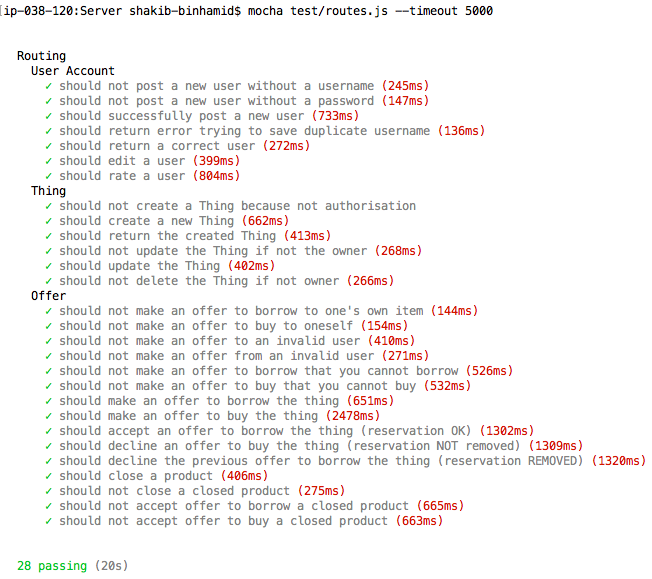
\includegraphics[height = \textwidth, width=\textwidth, keepaspectratio]{routes-test}
    \caption{REST API Behaviour Test}
    \label{fig:rest-test}
\end{figure}

\subsection{Database Integrity Test}

These tests go through each object (\textit{document} in this case) in the database. It then validates the referenced objects and constraints on their fields. For example: in Figure \ref{fig:db-test}, a test fails to find a reservation for a Thing, an offer/request for which was accepted. It means that the offer that it was reserved to is \textit{missing} and the Thing needs to be mended. Note that the actual \textit{fixing} is \textit{not} automated, rather I used these tests to monitor the database.

\begin{figure}[!h]
    \centering
    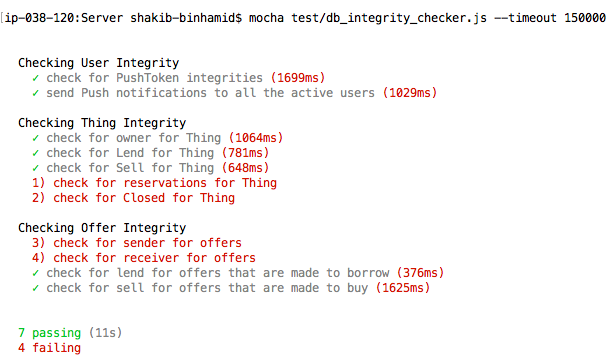
\includegraphics[height = \textwidth, width=\textwidth, keepaspectratio]{db-check}
    \caption{DB Integrity Check}
    \label{fig:db-test}
\end{figure}

\begin{figure}[!h]
    \centering
    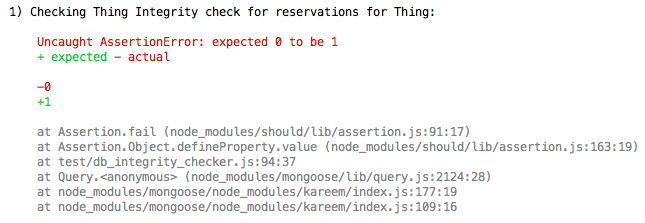
\includegraphics[height = \textwidth, width=\textwidth, keepaspectratio]{error}
    \caption{Error in Testing}
    \label{fig:error}
\end{figure}

The database integrity tests were also performed each sprint. In fact, these tests proved to be so helpful, that I ran them atleast once a development day. I imagine the tests to pave a path to future monitoring mechanism that may be put in place.\\

\section{Client Test}

It was not possible to make automated GUI tests for the client app for the following reasons - 

\begin{itemize}
	\item Touch-event mocking is not possible in Ionic
	\item Ionic libraries cannot be isolated
	\item AngularJS can usually be mocked, but Ionic integrates AngularJS, so it cannot be extracted either
\end{itemize}

In short, BDD or TDD is not possible, because the Ionic framework does not support such features. Even the community is silent in this regard. In fact, as discussed in Chapter \ref{chap:lit} in detail, this is a common problem across mobile app development, specially hybrid apps. I believe the reasons are - 

\begin{itemize}
	\item Ionic is undergoing a complete overhaul for version 2. So, the developers are mostly ignoring the current version.
	\item The production hybrid apps have proprietary, in-house test environments such as in Facebook etc.
\end{itemize}

As a result, I tested the client app regularly against pre-defined set of use case scenarios during development and with end users during UX evaluation.

\subsection{GUI Testing}

To test the GUI, I have exhaustively listed all the use case scenarios in Appendix \ref{appendix:gui-test}. This was built up as each feature had been added. At every sprint, I walked through every scenario multiple times, on two different Android mobiles - Moto X 1st Gen and Moto X Play. I used the list as my primary guide in client app testing. The list is comparable to a 100\% coverage of BDD testing on client.


\subsection{User Evaluation}

I have also evaluated the client app with the end users. More about this is discussed in Chapter \ref{chap:user}, Appendix \ref{appendix:interview} and \ref{appendix:ux}.
\chapter{User Participation}
\label{chap:user}

In this chapter, I discuss why and how I have interviewed the potential users of the app, as well as my experiences in doing so.

\section{Reason}

Even though I had a vision of what the app could be, the specific user stories must be structured and prioritised \textit{only} to the \textit{end users'} needs. So, the first round of interviews were run to empathise with my users' pain points. For example - I asked the users - \textit{Which of these features are more important to you and in what order and why such order?} (Appendix \ref{sec:interview1}), and the response dictated where I needed to concentrate. This idea stems from the simple fact that - "those affected by a design should have a say in the design process" \cite{Bjogvinsson:2012}. In fact, I turned the responses into user stories in backlog (See Chapter \ref{chap:proj-org}) and their pain points allowed me to prioritise them.\\

I also felt it necessary to define UX goals (e.g. evaluate navigation and white space use etc.) and run interactive interviews with the \textit{end users}. It is because users typically interact with mobile apps very differently to their desktop counterparts (e.g. average user spends about an hour a day on apps, whereas each session only lasts around a minute! \cite{Bohmer:2011}). So, even established assumptions about interaction often falls behind \cite{Sullivan:2013}. Responses to questions like - \textit{How do you know if someone responded to the ’x’ you posted earlier?} (Appendix \ref{sec:interview2}) pointed out some obvious faults in the app during UX evaluation when they could not complete the task in expected time or take the expected navigation route. I turned the issues into estimated work items (Appendix \ref{appendix:ux}) and fixed them in the following sprint.\\

\section{Methodology}

For each user participation period, I defined a goal first e.g. gain a better understanding of sharing economy between students in UoS and produce wireframes for RE period. Then a data collection method (e.g. interview, questionnaire, focus group, observations etc.) was chosen. I chose individual structured interviews with consented audio recording, physical notes and observation for qualitative data. I also asked them to speak aloud what they were thinking or doing. This method was chosen because video recording is time consuming and difficult to get \textit{right}, questionnaires often remove empathy and focus groups proved difficult to organise \cite{Arhippainen:2003}. I also believed qualitative data will provide more information than quantitative for my purposes.\\

Then I made interview scripts (with generally open ended approach to the questions), estimated time taken, applied for ethical approval with consent form and data protection guarantee. The notes taken were cross checked with the recorded audio for each individual afterwards. Data was kept secure on my personal laptop. It was then turned into user stories and prioritised based on observation. I also used the information to confirm prior assumptions.

\section{Experiences in RE}

I found two very distinct groups of interviewees in my first interview period - one group will express themselves a lot more than the others, rarely there was an \textit{ideal} persona. So, it soon proved difficult to keep track of the structured questions as the answers would often overlap or that there was barely any data from certain interviewees. As a result, interviews almost always ran overtime than what was estimated.\\

The planned interactive wireframing session, where users draw out how they believed their most desired features would be implemented, was very successful and productive. Every interviewee engaged easily and provided me with crucial ideas on how to structure UI elements and implement navigation. Similar experiences with card sorting technique, where they prioritised the important featured, which helped me prioritise user stories even in later stages.\\

I had also found it extremely helpful to have a very early prototype running on the mobile device \cite{Kangas:2005} that I used to develop the app, even during RE session. It gave a better perspective about wireframing to both the participants and I, and removed the usual gulf between the two parties \cite{Vermeeren:2010}.

\section{Experiences in UX Evaluation}

I had corrected my approach to the interview questions based on previous the experiences and made them slightly more specific and task based so as to keep the interviewees focused. Resultantly, the sessions ran almost exactly as long as they were estimated to run.\\

Very simple bugs, some of which I was aware of but never fixed because they were not prioritised (e.g. reverse chronological ordering of products etc.), distracted the participants from main tasks. Although they could have been fixed in between different sessions, I did not do so as it would jeopardise the study. In future, I will fix all the simple and obvious bugs before I run evaluation sessions.\\

The results from the sessions were very satisfactory. In general, the participants found the interface to be \textit{intuitive}, \textit{fun} and \textit{easy} to navigate. They also found the information layout to be \textit{clean} and animations to add \textit{life} to the app.\\

There were 10 easily fixable (1-2 hours) and 4 much harder to fix (more than 10 hours) issues found (see Appendix \ref{appendix:ux}). Most of these (9/10 of the former, 2/4 of the latter) were addressed in the sprint that followed soon after. I can truly appreciate the importance of user evaluation at this point and would recommend doing so at least after every two iterations in any future work.
\chapter{Evaluation \& Future Work}

In this chapter, I discuss how well the project went, which parts can be improved upon, what is left to complete as well as how others can use the results of the project in their own work.

\section{Project Success}

The selection of technologies proved to be very satisfactory. Interaction between the client and the server using JSON was made seamless due to full stack JavaScript development. The frameworks' community support was generally helpful, albeit their own rapid development made version specific support tedious. It was very easy to add new modules and libraries using \texttt{npm} and access mobile hardware plugin support by Ionic. Overall, fast prototyping was possible using the frameworks, as expected.\\

I believe that running the user interviews was a great success. I now have practical knowledge of how to prepare for such sessions, the methodology of interviews and observations and most importantly, interpreting the results. As found in the literature, it is extremely important to evaluate a prototype often; in my opinion - at least once every two sprints. This removes tunnel vision, sets realistic goals and prioritises the remaining work or bugs.\\

The server has been sufficiently tested with automated test suits, as discussed in Chapter \ref{chap:test} and the client was tested by scenerios and user interviews. This is satisfactory for a prototyping project within these time constraints.\\

Finally, the project organisation was a success. Development started early and finished a little over a week earlier than planned. Sprints were regularly reviewed, backlog was managed throughout the development period and bugs were documented. I believe that the app has reached an alpha stage, where there are a number of bugs and a few features are missing, but it is ready to be field tested and will reach feature-lock and beta in 3-4 iterations. 

\section{Points of Improvement}

The server was not satisfactorily \textit{unit} tested, while the Ionic framework provides none to very little support in automated testing in general. If this were to be a production ready service, I would, at least, rebuild the server in TDD style.\\

Push notification support is poor in \textit{every} hybrid app framework. The current choice of libraries is quite helpful, but will likely require some rewriting themselves to suit this app's needs. There needs to be a better guarantee of the delivery of the notifications.\\

Data models can be made simpler in the server. For example: Lend and Sell objects can be integrated in Thing, PushToken should be absorbed in User etc. This structure was chosen at first to prevent certain fields to be retrieved. In fact, later I discovered that the \texttt{mongoose} library natively provides methods that perform the intended behaviour. So, it is no longer necessary to separate the objects.\\

Finally, as a production-ready app, a paid Amazon S3 database should be chosen and integrated with the server to store images as BLOBs, rather than Base64 strings. This removes a large overhead from the main database.

\section{Future Development}

The app must have an improved rating system for the users, for example: there should be sub-ratings, e.g. timeliness, care-of-product etc. This project focused on the overall app, but a production-ready community driven app will heavily depend on a detailed and reliable rating system. In fact, some user research may be performed about how such a system may work before development.\\

Next, the in-app communication should be implemented. This could be done using the university email service, regular chatting frameworks, sms-call systems etc.\\

Finally, the app should have an automated recommendation notification system for desired items (wish-list) for the users. This feature should not require any additional frameworks, but such \textit{recommendation} system is usually difficult to get \textit{right}. Research should also be done on how similar systems handle the UX on client, e.g. Amazon or EBay.

\section{Usefulness in Other Projects}

The client app structure, feature list and server models can provide a useful framework for software projects that have community driven interaction models, e-commerce etc. They can also use the project plan or sprint times from the Gantt chart. Hopefully, it will also convince mobile app developers to invest resources in user interaction sessions.\\

This project has used technologies from various paradigms which can influence other projects. For example: student projects with asynchronous servers can get guidelines from the nodejs code, RESTful api developers can benefit from the relevant parts in server, app developers can also benefit enormously from the ionic project structure etc.
\chapter{Conclusion}
\label{chap:conclusion}

Even though \textit{Software Engineering} itself is now considered an established and mature study, application development for smartphones is a recent and diverse addition in the industry. Because of the wide variety of smartphones used by the people, there is also a plethora of development toolkits available for multiple different platforms. Although each major mobile OS has its own distinct engineering practices and architectural patterns, it is expected that an app is to be implemented and supported well simultaneously for multiple platforms. This project has tried to tackle the problem by using hybrid technologies to develop a mobile app.\\

It is also extremely difficult to rigidly define mobile app requirements in this volatile industry and satisfy user experiences for multiple platforms at the same time. I have successfully used scrum (iterative development and review) to develop the app, and organised interview sessions to engage the end-users in requirements elicitation, design and evaluate the app in hopes to evade such difficulties.\\

However, the benefits of fast development and multi-platform support comes with the price of automated testing on client side. While there are established practices in server building using NodeJS, apps built with such hybrid client frameworks as Ionic are nearly impossible to unit test because of lack of mocking and isolation support. In fact, there seems to be very few, if any, example of community support in this regard. This is certainly a barrier, but given the aims of the project, the issue can be considered a discovery of fact, rather than a major shortcoming.\\

Finally, I consider the project to be successful, and valuable for future students, because it demonstrates relevant agile software development processes such as scrum, daily testing, evolving user stories etc. within the short project frame, experiments with emergent technologies in mobile app industry and evaluates the results against end users' expectations.

%% bibliography
\addcontentsline{toc}{chapter}{Bibliography}
\bibliography{references}

%% appendix
\appendix
\chapter{Read Me}

This project was done using a Macbook Air Mid 2012 with Mac OS X 10.11 El Capitan. So, the following guide is confirmed to work on such a system.\\

However, it should work without any changes on a recent Unix based system and with slight changes on Windows. The framework websites provide more knowledge on platform specific issues.\\

The following sections must be completed in order.

\section{Install Node.JS}

First install the \texttt{node.js} runtime from \texttt{\hyperref[https://nodejs.org/en/]{https://nodejs.org/en/}}. This will also install the package manager \texttt{npm}. On the development system it was \texttt{0.12.7}.\\

You can update existing versions using \texttt{sudo npm install npm -g}. Also, check the current version using \texttt{node --version}.

\section{Install Express.JS}

Use \texttt{sudo npm install -g express}. The \texttt{-g} option installs the package globally. This is necessary to start the server locally.

\section{Add Database}

This project only used a remote database on mLab at \texttt{\hyperref[https://mlab.com]{https://mlab.com}}. Create a free account here, add a database, add a \textit{db user} and take note of the username-password. On mLab, over at your database page, you should see the \textit{db URI}. Fill in the username-password and overwrite \texttt{server.js} and \texttt{test/config-debug.js} at the Server project root.

\section{Install Heroku Toolbelt}

If you are using Heroku, as was used in this project, then you must install the Heroku Toolbelt from \texttt{\hyperref[https://toolbelt.heroku.com]{https://toolbelt.heroku.com}}.

\section{Heroku Deploy}

Once you have created a Heroku account (free), \texttt{cd} over to the \textit{Server} project root. Then use \texttt{heroku login} to log into your account from CLI. The server \textit{must} be a \textit{git} repository. If it is not, use \texttt{git init} to create one.\\

Use \texttt{heroku create <app-name>} where \texttt{<app-name>} is what you want to call your server. This will add a \textit{Heroku git remote}.\\

Finally, use \texttt{git push heroku master} to push the \texttt{master} branch to Heroku. It will now be deployed to \texttt{<app-name>.herokuapp.com}.\\

You can use \texttt{heroku logs --tail} to see real-time logs from your remote server.

\section{Server local}

Use \texttt{npm install} while in the Server project root. It will install all the modules (including dev-dependencies) from \texttt{package.json}.\\

Finally, use \texttt{node server.js} to run the server. You should install \textit{nodemon} by \texttt{sudo npm install -g nodemon} to automatically restart the server on code change.

\section{Install Ionic \& Cordova}

Use \texttt{sudo npm install -g cordova ionic} to install both Ionic and Cordova CLI.\\

It is recommended that you use \texttt{Google Chrome} as your \textit{default} browser.

\section{Add Platforms to Ionic Project}

Apart from \textit{Android}, which should already be added to the project in the source code provided, you can add other platforms. For example, to add iOS, use \texttt{ionic platform add ios}.\\

You \textit{must} install Android Studio from \texttt{\hyperref[http://developer.android.com/sdk/index.html]{http://developer.android.com\\/sdk/index.html}} to build for Android and XCode from\\ \texttt{\hyperref[https://developer.apple.com/xcode/download/]{https://developer.apple.com/xcode/download/}} to build for iOS.

\section{Install Plugins \& Ionic Libraries}

To add plugins for a platform, first add the platform, then use \texttt{ionic plugin add <plugin>}. Replace \texttt{<plugin>} with cordova-plugin-device, cordova-plugin-console, cordova-plugin-whitelist, cordova-plugin-splashscreen, cordova-plugin-statusbar, ionic-plugin-keyboard, com-badrit-base64, cordova-imagePicker.git, cordova-plugin-file. Use these \textit{one by one}.\\

Some might already be installed depending on your Ionic version. If they are, just ignore and carry on.\\

You can also perform \texttt{ionic state reset} to re-download all the plugins from \texttt{package.json} file of your Ionic project.

\section{Add GCM API Key}

Create a Google account, go to \texttt{\hyperref[https://console.developers.google.com]{https://console.developers.google.com}}, create a project. Add \textit{GCM} as an API, create a \textit{Server Key} and take note of it.\\

Then update \texttt{controllers/offer.js} and add your GCM API key.

\section{Set up Ionic Push}

Push is not supplied as a standard with Ionic. Create an Ionic account. Look at \texttt{\hyperref[http://docs.ionic.io/v1.0/docs/push-android-setup]{http://docs.ionic.io/v1.0/docs/push-android-setup}} for GCM integration in Ionic.\\

In essence, use \texttt{ionic add ionic-platform-web-client} on the Client project root. Then \texttt{ionic push --google-api-key <your-google-api-key>} and \texttt{ionic config set gcm\_key}\\ \texttt{<your-gcm-project-number>}. Head over to \texttt{\hyperref[http://apps.ionic.io]{http://apps.ionic.io}}, log in using your ionic account and you will see your push service connected with your app.

\section{Change Host id in Client}

Open up \texttt{<clinet-project-root>/www/js/services.js} and change \texttt{routes.APP} to your server app address. You can also toggle \texttt{development} to access either the local server or the remote one.

\section{App Build}

\texttt{cd} to Client project root. Set \texttt{development} is set to \texttt{false} in \texttt{services.js}. Once you have added the desired platform and plugins (and platform SDK), use \texttt{ionic build <platform>} to build an installer for the platform.\\

For android, a \texttt{android-debug.apk} file will be created at \texttt{/platforms/\\android/build/outputs/apk/}. Transfer the file over to the mobile and install it.

\section{App local}

Disable web-security to allow cross origin policies in chrome. Look online for you platform specific instruction. Otherwise, your app cannot receive data in browser emulation. At Client project root, use \texttt{ionic serve -l} to deploy both iOS and Android emulation.
\chapter{Libraries Used}
\label{appendix:libs}

\newcommand{\link}[1]{\url{#1}}

Below is the complete list of libraries, frameworks that were used in any way in the project and their github source links - 

\begin{description}
	\item [Ionic Framework] v.1.1.1 by \textit{Drifty Co} \\ \link{https://github.com/driftyco/ionic}
	\item [AngularJS] v.1.4.3 by \textit{Google} \\ \link{https://github.com/angular/angular.js}
	\item [Phonegap base64] v.0.2.0 by \textit{Hazem Hagrass} \\ \link{https://github.com/hazemhagrass/phonegap-base64}
	\item [Cordova ImagePicker] v.1.1.0 by \textit{Wymsee} \\ \link{https://github.com/wymsee/cordova-imagePicker}
	\item [Cordova Datepicker] v.0.9.3 by \textit{Vitalii Blagodir} \\ \link{https://github.com/VitaliiBlagodir/cordova-plugin-datepicker.git}
	\item [Phonegap Plugin Push] v.1.5.3 by \textit{Adobe PhoneGap Team} \\ \link{https://github.com/phonegap/phonegap-plugin-push.git}
	\item [Angular UI Router] v.0.2.7 by \textit{Angular UI Team} \\ \link{https://github.com/angular-ui/ui-router.git}
	\item [Ionic Material] v.0.4.0 by \textit{Zach Fitzgerald} \\ \link{https://github.com/zachsoft/Ionic-Material/}
	\item [Ionic Rating] v.0.1.0 by \textit{Fraser Xu} \\ \link{https://github.com/fraserxu/ionic-rating.git}
	\item [ngCordova] v.0.1.23-alpha by \textit{Drifty Co} \\ \link{https://github.com/driftyco/ng-cordova.git}
	\item [NodeJS] v.0.12.7 by \textit{NodeJS Foundation} \\ \link{https://github.com/nodejs/node}
	\item [ExpressJS] v.4.13.3 by \textit{TJ Holowaychuk} \\ \link{https://github.com/strongloop/express.git}
	\item [MongooseJS] v.4.2.2 by \textit{Guillermo Rauch} \\ \link{https://github.com/Automattic/mongoose/}
	\item [Mongoose Deep Populate] v.2.0.3 by \textit{Buu Nguyen} \\ \link{https://github.com/buunguyen/mongoose-deep-populate.git}
	\item [Node GCM] v.0.13.0 by \textit{Marcus Farkas} \\ \link{http://github.com/ToothlessGear/node-gcm}
	\item [PassportJS] v.0.2.2 by \textit{Jared Hanson} \\ \link{https:////github.com/jaredhanson/passport.git}
	\item [Mocha] v.2.3.4 by \textit{MochaJS} \\ \link{https://github.com/mochajs/mocha}
	\item [ShouldJS] v.8.0.2 by \textit{TJ Holowaychuk} \\ \link{https://github.com/shouldjs/should.js.git}
	\item [Supertest] v.1.1.0 by \textit{TJ Holowaychuk} \\ \link{https://github.com/visionmedia/supertest.git}
\end{description}

\chapter{Interview Scripts}
\label{appendix:interview}
\section{Interview 1}
\label{sec:interview1}
\begin{itemize}
	\item What items do you own, but not use often (Once a week or less)?
	\item Which of these items would you share with others?
	\item Why those items and not the others? (If none, then why?)
	\item If another student were to borrow your item, which items - 
		\begin{itemize}
			\item Would you have them pay for i.e. sell? Why?
			\item Would you have them put a deposit for? Why?
			\item Would you make them share an item of their own for i.e. swap? Why?
			\item Would you let them borrow regardless? Why?
			\item Anything else you have to add?
		\end{itemize}
	\item How much does trusting the borrower or lender get in these decisions?
	\item Tell me how you would increase trust in the community to share your belongings?
	\item How can the borrower increase the trust?
	\item How can the lender increase the trust?
	\item How would you go about \& carry out the transaction? How would set up how and where to meet or post?
	\item What would you expect to see in as you open the application? 
	\item What would you want to do first after you open it? 
	\item What other functions would you perform as a user? As a borrower ? As a sharer? 
	\item Which of these features are more important to you and in what order and why such order? 
	\item How would you perform the top 3 features that you have selected? (Ask them to draw out a flowchart like steps for the functions) 
\end{itemize}

\section{Interview 2}
\label{sec:interview2}
\begin{itemize}
	\item {You have just installed the app. You open it for the first time.
		\begin{itemize}
			\item What do you see?
			\item What do you want to do now?
		\end{itemize}
		}
	\item {
		\begin{itemize}
			\item Navigate back to the home page. (steps \& time)
			\item Try to find your profile. How else could you find your profile? (steps \& time)
		\end{itemize}
		}
	\item You want to post this 'x' on the community to sell, but you also don't mind lending it. What do you do? (steps \& time)
	\item You're looking for a used 'macbook' to buy. How will you find it? (steps \& time)
	\item You've found a 'moto x'. You can use it for your project. How can you borrow it? (steps \& time) What do you think happens next?
	\item You want to find out more about the item or its seller. How? (steps \& time)
	\item How do you know if someone responded to the 'x' you posted earlier? Find such responses on the app. (steps \& time)
	\item You want to accept a request. How? What do you think happens when you accept?
	\item You want to decline a request. How? What do you think happens when you decline a request?
	\item Note 2 points that could be 'improved' in the app.
	\item Note 2 points that the app does well. 
\end{itemize}
\chapter{Gantt Charts}
\label{appendix:gantt}

\begin{figure}[!h]
    \centering
    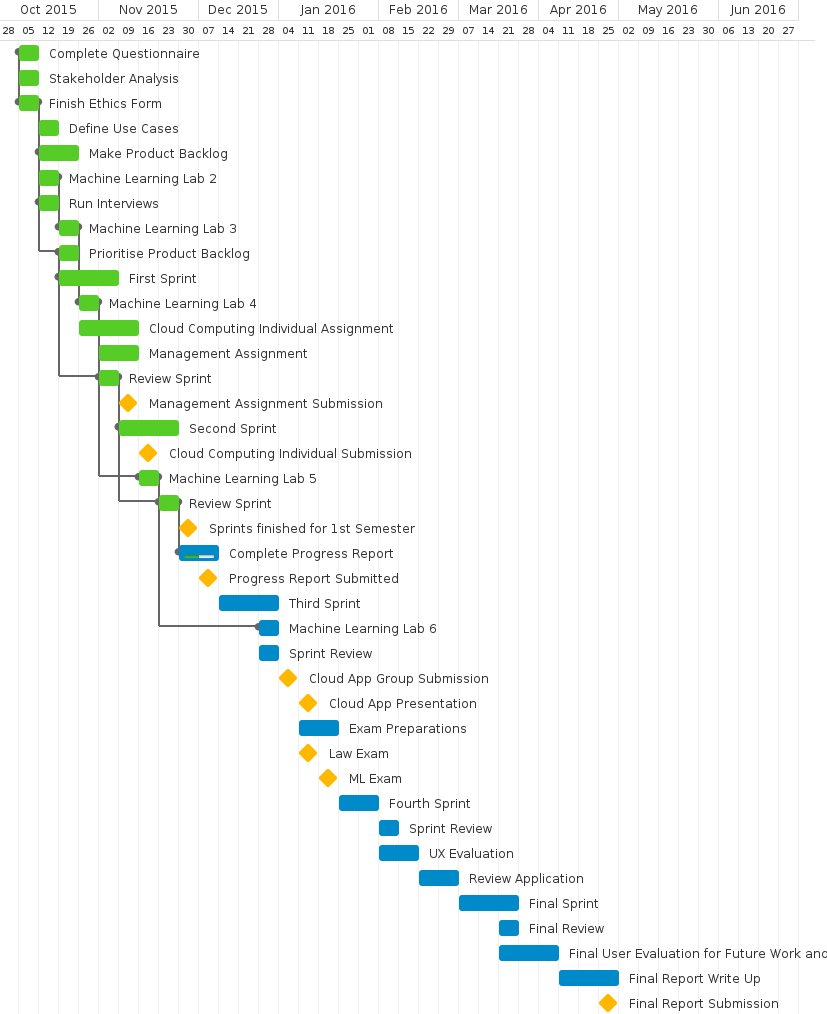
\includegraphics[height = 1.3\textwidth, width= \textwidth, keepaspectratio]{gantt-v1}
    \caption{Initial Gantt Chart}\label{fig:gantt-v1}
\end{figure}

\begin{figure}[!h]
    \centering
    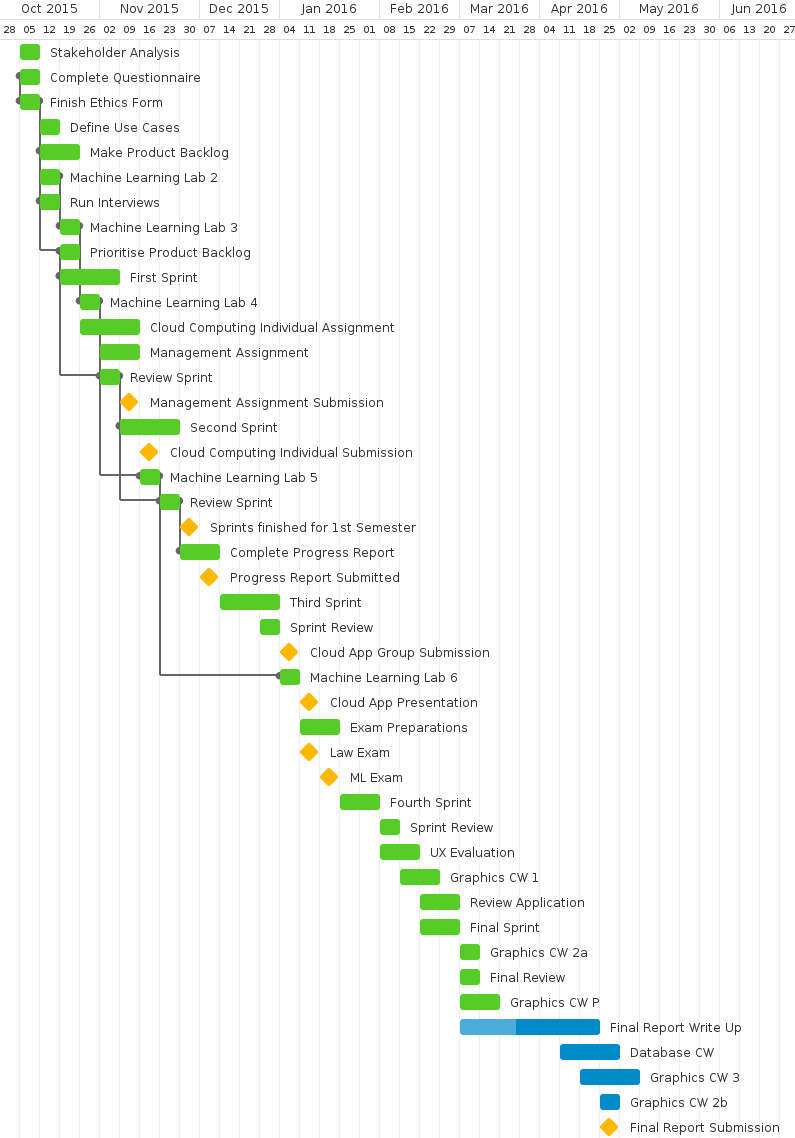
\includegraphics[width= \textwidth, keepaspectratio]{gantt-v2}
    \caption{Final Gantt Chart}\label{fig:gantt-v2}
\end{figure}
\chapter{UX Results}
\label{appendix:ux}

\definecolor{agree}{RGB}{0, 122, 0}
\definecolor{disagree}{RGB}{122, 0, 0}
\definecolor{niceButWontCol}{RGB}{222, 222, 0}
\definecolor{toughCol}{RGB}{222, 100, 0}
\definecolor{fixableCol}{cmyk}{0, 0.208, 0.0429, 0.1412}

\newcommand{\tab}{\vspace{0.5cm}}
\newcommand{\username}[1]{\textsc{\textbf{#1}}}
\newcommand{\user}[1]{\item[\username{#1}] \hfill}
\newcommand{\agrees}[1]{\color{agree}\username{#1}\color{black}}
\newcommand{\disagrees}[1]{\color{disagree}\username{#1}\color{black}}
\newcommand{\fixable}[1]{\colorbox{fixableCol}{#1}}
\newcommand{\tough}[1]{\colorbox{toughCol}{#1}}
\newcommand{\cant}[1]{\colorbox{niceButWontCol}{#1}}

\small
\begin{center}
	\fixable{fixable easy (1-2 hrs)} \tough{necessary but tough (\textgreater 10 hrs)} \cant{nice but cant}
\end{center}
\begin{itemize}
	\item {You have just installed the app. You open it for the first time.
		\begin{itemize}
			\item What do you see?
					\begin{itemize}
						\item List of products \agrees{1}, \agrees{2} - ads, \agrees{4}, \agrees{5}
						\item \fixable{Expected the products in reverse chronological order} \agrees{4}
						\item Gray boxes. \agrees{3}
						\item Details of products. \agrees{2}, \agrees{5}
						\item Would rather not have a placeholder image for items without an image \agrees{1}, \disagrees{4} 	
						\item Pictures are a bit small. \agrees{5}
						\item Circle buttons on bottom were getting in the way. \agrees{1}, \agrees{2}, \disagrees{3}, \disagrees{5}
						\item \tough{Expected to have a category section} \agrees{2}, \agrees{3}, \agrees{4}				
						\vspace{0.5cm}
						
						\item GIF avatars of people \agrees{1}, \agrees{3}, \agrees{4}
						\item \fixable{Expects clicking on the user avatar on product card to bring up the user profile} \agrees{1}
						\item \fixable{Expected owner's name to be on the product card along with their avatars} \agrees{4}
						\vspace{0.5cm}
						
						\item Can see a nice chat option \agrees{1} 
						\item Borrow / buy is disabled means those options not available for the product \agrees{1} 
						\item Good that can't borrow own things \agrees{1} 
						\item Some items are closed seeing the red tag. \agrees{2}, \agrees{4}, \agrees{5}
						\vspace{0.5cm}
						
						\item Search bar for finding products. \agrees{2}, \agrees{3}
						\item Wasn't sure what the blue person icon meant. \agrees{4}
						\item \cant{Expected to have a tutorial to explain the basic usage} \agrees{4}
					\end{itemize}
			\item What do you want to do now?
				\begin{itemize}
					\item Search for something. \agrees{3}, \agrees{1}
					\item Click on a product. \agrees{1}, \agrees{2}, \agrees{3}, \agrees{4}
					\item Add a product. \agrees{1}, \agrees{5}
				\end{itemize}
		\end{itemize}
		}
		\tab
	\item {
		\begin{itemize}
			\item Navigate back to the home page. (steps \& time)
				\begin{itemize}
					\item Everyone started looking about the app and made their way back to the home page. This task was trivial.
					\item Navigation stack messed up in some order. Couldn't reproduce how they did it. \agrees{1}
				\end{itemize} 
			\item Try to find your profile. How else could you find your profile? (steps \& time)
				\begin{itemize}
					\item Everyone found the profiles before this question was asked. It was trivial.
					\item From the icon on home. \agrees{1}, \agrees{2}, \agrees{3}, \agrees{4}, \agrees{5}
					\item From the menu on the top left. \agrees{1}, \agrees{2}, \agrees{3}, \agrees{4}, \agrees{5}
					\item From one of own products. \agrees{3}
					\item Prefer the icon on home. \agrees{3}, \agrees{5}
					\item Prefer the menu option. \agrees{1}, \agrees{2}
					\vspace{0.5cm}
					
					\item Cannot change avatar. \agrees{1}
					\item Liked the idea of rating. \agrees{1}, \agrees{4}, \agrees{5}
					\item \fixable{Not sure if the comments are about the products, deals or person's own self}. \agrees{1}, \agrees{2}, \agrees{4}
					\item \tough{\tiny{Not sure what the ratings represent, i.e. expected to see granular ratings e.g. timeliness 4, care of product 3 etc}} \agrees{1}, \agrees{2}
					\item Good that can't rate oneself. \agrees{4}, \agrees{5}
					\item Rated someone. \agrees{3}, \agrees{5}
					\item Failed to rate someone. \agrees{1}
				\end{itemize}
		\end{itemize}
		}
		\tab
	\item You want to post this 'x' on the community to sell, but you also don't mind lending it. What do you do? (steps \& time)
		\begin{itemize}
			\item Everyone followed the expected route, filled in the fields and clicked the green tick. Took less than two minutes.
			\item Click on (+) on home page. \agrees{1}, \agrees{2}, \agrees{3}, \agrees{4}, \agrees{5}
			\item Likes the use of toggle buttons for sell or lend options. \agrees{5}
			\item Prefer to have types in defined categories. \agrees{3}, \agrees{4}
			\item Relates types to tags. \agrees{4}
			\item Easy to add and see the scrollable picture. \agrees{1}, \agrees{5}
			\vspace{0.5cm}
			\item \tough{\footnotesize{Noticed the lending bug - where things are always put on for sale and lending regardless of options}}
			\item \fixable{Expected a confirmation} \agrees{4}
			\item \fixable{Expected to be taken to the summary page} \agrees{5}
			\item \fixable{Expected the product to be on top of the list} \agrees{1}, \agrees{2}, \agrees{3}, \agrees{4}, \agrees{5}
		\end{itemize}
		\tab	
	\item You're looking for a used 'macbook' to buy. How will you find it? (steps \& time)
		\begin{itemize}
			\item Trivial to search for a product on the home page (less than 30 seconds). But not trivial to get out of the search.
			\item \cant{Search doesn't work on types or wrongly spelt names etc}. \agrees{3}, \agrees{4}, \agrees{5}
			\item \fixable{Expected to see a message or suggestions when no results for a search were found} \agrees{1}, \agrees{2}, \agrees{3}, \agrees{4}
			\item Liked the cross to clear the search field. \agrees{3}, \agrees{4}, \agrees{5}
		\end{itemize}
		\tab
	\item You've found a 'moto x'. You can use it for your project. How can you borrow it? (steps \& time) What do you think happens next?
		\begin{itemize}
			\item Trivial to borrow an item. Less than 30 seconds.
			\item Click on borrow button if available. \agrees{1}, \agrees{2}, \agrees{3}, \agrees{4}, \agrees{5}
			\item If not available to borrow, contact the user via chat. \agrees{3}
			\item Expected to have the options on the product page too. \agrees{2}, \agrees{5}
			\item Buyer gets notified. \agrees{1}, \agrees{2}, \agrees{3}, \agrees{4}, \agrees{5}
			\item Item was reserved. \agrees{2}, \agrees{3}, \agrees{4}
			\item Get in touch with the buyer and exchange. Then complete. \agrees{1}, \agrees{3}, \agrees{4}
			\item Complete immediately. \agrees{2}, \agrees{5}
			\item \cant{Products should be considered closed if both parties complete it} \agrees{4}
		\end{itemize}
		\tab
	\item You want to find out more about the item or its seller. How? (steps \& time)
		\begin{itemize}
			\item Trivial. Found within 30 seconds. Comments about own profile applies here too.
			\item Went to product details page, then owner name. \agrees{1}, \agrees{2}, \agrees{3}, \agrees{4}, \agrees{5}
			\item \fixable{\footnotesize{Expected the closed items on a product to be marked on a profile page like on the cards}} \agrees{4}, \agrees{5}
		\end{itemize}
		\tab
	\item How do you know if someone responded to the 'x' you posted earlier? Find such responses on the app. (steps \& time)
		\begin{itemize}
			\item The most difficult task here. Took quite a bit of looking around. More than 60 seconds.
			\item Expected to get a notification (didn't always get sent a notification because of Google servers). \agrees{1}, \agrees{2}, \agrees{3}, \agrees{4}, \agrees{5}
			\item Found on product details page. \agrees{1}, \agrees{2}, \agrees{4}, \agrees{5}, \disagrees{3}
			\item \tough{Expected to find separate place on profile for notifications about such things} \agrees{1}, \agrees{2}, \agrees{3}, \agrees{4}, \agrees{5}
			\item Expected to have a tab on the menu for notifications directly. \agrees{4}, \agrees{5}
		\end{itemize}
		\tab
	\item You want to accept a request. How? What do you think happens when you accept?
		\begin{itemize}
			\item Trivial and took less than 30 seconds.
			\item Click on accept button on an offer. \agrees{1}, \agrees{2}, \agrees{3}, \agrees{4}, \agrees{5}
			\item The other side gets notified. \agrees{1}, \agrees{2}, \agrees{3}, \agrees{4}, \agrees{5}
		\end{itemize}
		\tab
	\item You want to decline a request. How? What do you think happens when you decline a request?
		\begin{itemize}
			\item Trivial. Similar to above.
		\end{itemize} 
		\tab 
		
	\item Note 2 points that could be 'improved' in the app.
		\begin{itemize}
			\item Add meaning to rating \agrees{1}
			\item Improve the interaction with a failed search and make clearing a search better \agrees{1}
			\vspace{0.5cm}
			\item Make notifications clearer to find. \agrees{2}, \agrees{3}, \agrees{5}
			\item Make scrolling better. \agrees{2}
			\vspace{0.5cm}
			\item Add categories for products. \agrees{3}
			\item Separate tab in the menu for own products \agrees{5}
			\vspace{0.5cm}
			\item \fixable{Add time tag to comments}
			\item Order of products in reverse chronological order.
		\end{itemize}
		\tab 
	\item Note 2 points that the app does well.
		\begin{itemize}
			\item Product card layout is clean with three buttons for obvious actions. \agrees{1}, \agrees{3}
			\item Intuitive and clean interface. \agrees{2}, \agrees{4}, \agrees{5}
			\item Animations, loading, fluidity adds life to the app. \agrees{4}
			\item Adding pictures of products is easy, necessary and done well. \agrees{1}
		\end{itemize}		 
\end{itemize}
\chapter{GUI Testing}
\label{appendix:gui-test}

\normalsize
Table \ref{table:gui-test1}, \ref{table:table:gui-test2}, \ref{table:table:gui-test3}, \ref{table:table:gui-test4} and \ref{table:table:gui-test5} contains a comprehensive list of the GUI tests that were performed by the end of development. It accounts for the expected behaviour, resultant behaviour and the possible bug in the system.

\newcolumntype{b}{X}
\newcolumntype{s}{>{\hsize=.3\hsize}X}

\small
\begin{sidewaystable}
\centering
    \begin{tabularx}{\textwidth}{cbbbcb}
    \toprule
    \centering
    \emph{\textbf{\#}} & \emph{\textbf{Scene}} & \emph{\textbf{Expected}} & \emph{\textbf{Actual}} & \emph{\textbf{Accept}} & \emph{\textbf{Bug}} \\
    \midrule
    \texttt{1}
    		& Open the app and stay on login page
    		& The background to show up
    		& OK, but takes some time
    		& Y
    		& -- \\
    		\cline{3-6} \noalign{\smallskip}
    		&& Labels on top, password covered, form filled
    		& Labels misplaced on first login, rest OK
    		& Y
    		& Label stays on textfield without focus on first login \\
    \midrule
    \texttt{2}
    		& Login
    		& Taken to product list
    		& OK
    		& Y
    		& -- \\
    \midrule
    \texttt{3}
    		& Products page examination
    		& Reverse chronology of products
    		& OK
    		& Y
    		& -- \\
    		\cline{3-6} \noalign{\smallskip}
    		&& Pull to refresh
    		& OK
    		& Y
    		& --\\
    		\cline{3-6} \noalign{\smallskip}
    		&& Only latest 20 at first
    		& OK
    		& Y
    		& --\\
    		\cline{3-6} \noalign{\smallskip}
    		&& Closed products at bottom
    		& OK
    		& Y
    		& --\\
    \midrule
    \texttt{4}
    		& Product card examination
    		& Owner's avatar, name, date
    		& OK
    		& Y
    		& -- \\
    		\cline{3-6} \noalign{\smallskip}
    		&& user avatar goes to profile
    		& OK
    		& Y
    		& --\\
    		\cline{3-6} \noalign{\smallskip}
    		&& item name, description, picture, options
    		& OK
    		& Y
    		& --\\
    		\cline{3-6} \noalign{\smallskip}
    		&& Offer buttons disabled or enabled appropriately
    		& OK
    		& Y
    		& --\\
    		\cline{3-6} \noalign{\smallskip}
    		&& Default picture
    		& OK
    		& Y
    		& --\\
    		\cline{3-6} \noalign{\smallskip}
    		&& Appropriate closed tag
    		& OK
    		& Y
    		& --\\
    \bottomrule
    \end{tabularx}
    \caption{GUI Testing after Sprint 5a}
    \label{table:gui-test1}
\end{sidewaystable}

\begin{sidewaystable}
\centering
    \begin{tabularx}{\textwidth}{cbbbcb}
    \toprule
    \centering
    \emph{\textbf{\#}} & \emph{\textbf{Scene}} & \emph{\textbf{Expected}} & \emph{\textbf{Actual}} & \emph{\textbf{Accept}} & \emph{\textbf{Bug}} \\
    \midrule
    \texttt{5}
    		& Side menu examination
    		& Profile takes to own profile
    		& OK
    		& Y
    		& -- \\
    		\cline{3-6} \noalign{\smallskip}
    		&& Categories takes to categories
    		& OK
    		& Y
    		& --\\
    		\cline{3-6} \noalign{\smallskip}
    		&& Request goes to offers
    		& OK
    		& Y
    		& --\\
    		\cline{3-6} \noalign{\smallskip}
    		&& Logout returns to login
    		& OK
    		& Y
    		& --\\
    	\midrule
    	\texttt{6}
    		& Add product button placement
    		& Floats on bottom right
    		& OK
    		& Y
    		& -- \\
    	\midrule
    	\texttt{7}
    		& New Product examination
    		& name required field
    		& OK
    		& Y
    		& -- \\
    		\cline{3-6} \noalign{\smallskip}
    		&& Can't add product without name
    		& OK
    		& Y
    		& --\\
    		\cline{3-6} \noalign{\smallskip}
    		&& Description resizable
    		& OK
    		& Y
    		& --\\
    		\cline{3-6} \noalign{\smallskip}
    		&& Lend and sell toggle options
    		& OK
    		& Y
    		& --\\
    		\cline{3-6} \noalign{\smallskip}
    		&& Lend date from today
    		& OK
    		& Y
    		& --\\
    		\cline{3-6} \noalign{\smallskip}
    		&& Picture from gallery
    		& OK
    		& Y
    		& --\\
    		\cline{3-6} \noalign{\smallskip}
    		&& Picture from camera
    		& OK
    		& Y
    		& --\\
    		\cline{3-6} \noalign{\smallskip}
    		&& Multiple Category
    		& OK
    		& Y
    		& --\\
    		\cline{3-6} \noalign{\smallskip}
    		&& Clear category on cancel
    		& Selection stays put
    		& N
    		& Scoped variable is not clearing\\
    \bottomrule
    \hline
    \end{tabularx}
    \caption{GUI Testing after Sprint 5b}
    \label{table:table:gui-test2}
\end{sidewaystable}

\begin{sidewaystable}
\centering
    \begin{tabularx}{\textwidth}{cbbbcb}
    \toprule
    \centering
    \emph{\textbf{\#}} & \emph{\textbf{Scene}} & \emph{\textbf{Expected}} & \emph{\textbf{Actual}} & \emph{\textbf{Accept}} & \emph{\textbf{Bug}} \\
    \midrule
    \texttt{7}
    		& New Product examination
    		& Lend and Sell done correctly
    		& Both selected always
    		& N
    		& Scoped variable not clearing on Lend \\
    		\cline{3-6} \noalign{\smallskip}
    		&& Cancel closes modal
    		& OK
    		& Y
    		& --\\
    \midrule
    \texttt{8}
    		& Search bar examination
    		& Correctly aligned, button disabled
    		& OK
    		& Y
    		& -- \\
    		\cline{3-6} \noalign{\smallskip}
    		&& Typing removes products
    		& OK
    		& Y
    		& --\\
    		\cline{3-6} \noalign{\smallskip}
    		&& Cross clears field
    		& OK
    		& Y
    		& --\\
    		\cline{3-6} \noalign{\smallskip}
    		&& Message for failed search
    		& OK
    		& Y
    		& --\\
    	\midrule
    	\texttt{9}
    		& New Product
    		& Added on top
    		& OK
    		& Y
    		& Y \\
    		\cline{3-6} \noalign{\smallskip}
    		&& confirmation given
    		& OK
    		& Y
    		& --\\
    \midrule
    \texttt{9}
    		& Product page examination
    		& Name, description, options, category
    		& OK
    		& Y
    		& -- \\
    		\cline{3-6} \noalign{\smallskip}
    		&& Owner links to profile
    		& OK
    		& Y
    		& --\\
    		\cline{3-6} \noalign{\smallskip}
    		&& Offers iff for own item
    		& OK
    		& Y
    		& --\\
    		\cline{3-6} \noalign{\smallskip}
    		&& Picture slide viewable
    		& OK
    		& Y
    		& --\\
    		\cline{3-6} \noalign{\smallskip}
    		&& Navigable back
    		& OK
    		& Y
    		& --\\
    \midrule
    \texttt{10}
    		& Loading examination
    		& Animation shown
    		& OK
    		& Y
    		& -- \\
    \bottomrule
    \hline
    \end{tabularx}
    \caption{GUI Testing after Sprint 5c}
    \label{table:table:gui-test3}
\end{sidewaystable}

\begin{sidewaystable}
\centering
    \begin{tabularx}{\textwidth}{cbbbcb}
    \toprule
    \centering
    \emph{\textbf{\#}} & \emph{\textbf{Scene}} & \emph{\textbf{Expected}} & \emph{\textbf{Actual}} & \emph{\textbf{Accept}} & \emph{\textbf{Bug}} \\
    \midrule
    \texttt{11}
    		& Profile examination
    		& Avatar, name displayed
    		& OK
    		& Y
    		& -- \\
    		\cline{3-6} \noalign{\smallskip}
    		&& Rating count \& average
    		& OK
    		& Y
    		& --\\
    		\cline{3-6} \noalign{\smallskip}
    		&& Cannot rate own
    		& OK
    		& Y
    		& --\\
    		\cline{3-6} \noalign{\smallskip}
    		&& Cannot rate 0
    		& OK
    		& Y
    		& --\\
    		\cline{3-6} \noalign{\smallskip}
    		&& Can rate others
    		& OK
    		& Y
    		& --\\
    		\cline{3-6} \noalign{\smallskip}
    		&& Comments in a list
    		& OK
    		& Y
    		& --\\
    		\cline{3-6} \noalign{\smallskip}
    		&& Own products list
    		& OK
    		& Y
    		& --\\
    		\cline{3-6} \noalign{\smallskip}
    		&& Products deletable if own
    		& OK
    		& Y
    		& --\\
    		\cline{3-6} \noalign{\smallskip}
    		&& Products not deletable if others'
    		& OK
    		& Y
    		& --\\
    		\cline{3-6} \noalign{\smallskip}
    		&& Products link to product page
    		& OK
    		& Y
    		& --\\
    		\cline{3-6} \noalign{\smallskip}
    		&& Navigable back
    		& OK
    		& Y
    		& --\\
    \midrule
    \texttt{12}
    		& Requests examination
    		& Recent requests first
    		& OK
    		& Y
    		& -- \\
    		\cline{3-6} \noalign{\smallskip}
    		&& Older requests separate
    		& OK
    		& Y
    		& --\\
    		\cline{3-6} \noalign{\smallskip}
    		&& Request notification
    		& Received most of the times
    		& Y
    		& GCM delivery unpredictable\\
    		\cline{3-6} \noalign{\smallskip}
    		&& Options correctly enabled or disabled
    		& OK
    		& Y
    		& --\\
    \bottomrule
    \hline
    \end{tabularx}
    \caption{GUI Testing after Sprint 5d}
    \label{table:table:gui-test4}
\end{sidewaystable}

\begin{sidewaystable}
\centering
    \begin{tabularx}{\textwidth}{cbbbcb}
    \toprule
    \centering
    \emph{\textbf{\#}} & \emph{\textbf{Scene}} & \emph{\textbf{Expected}} & \emph{\textbf{Actual}} & \emph{\textbf{Accept}} & \emph{\textbf{Bug}} \\
    \midrule
    \texttt{13}
    		& Requests examination
    		& Product name links to product page
    		& OK
    		& Y
    		& -- \\
    		\cline{3-6} \noalign{\smallskip}
    		&& Requester name and rating
    		& OK
    		& Y
    		& --\\
    		\cline{3-6} \noalign{\smallskip}
    		&& Request reason and date
    		& OK
    		& Y
    		& --\\
    		\cline{3-6} \noalign{\smallskip}
    		&& No request message
    		& OK
    		& Y
    		& --\\
    	\midrule
    \texttt{14}
    		& Categories examination
    		& Category buttons displayed
    		& OK
    		& Y
    		& -- \\
    		\cline{3-6} \noalign{\smallskip}
    		&& Search header displayed
    		& OK
    		& Y
    		& --\\
    		\cline{3-6} \noalign{\smallskip}
    		&& Failed search message
    		& OK
    		& Y
    		& --\\
    		\cline{3-6} \noalign{\smallskip}
    		&& Search results gives product cards
    		& OK
    		& Y
    		& --\\
    \bottomrule
    \hline
    \end{tabularx}
    \caption{GUI Testing after Sprint 5e}
    \label{table:table:gui-test5}
\end{sidewaystable}





















\end{document}